\documentclass[sigconf,balance=false]{aamas}

\usepackage{booktabs}
\usepackage{graphicx}
\usepackage{amsmath}

% Course report: suppress ACM conference/reference/copyright blocks.
\setcopyright{none}
\settopmatter{printacmref=false, printccs=false, printfolios=true}
\renewcommand\footnotetextcopyrightpermission[1]{}

\title[Low-Altitude Drone Logistics Scheduling]{A Collaborative Task Dispatching Platform for Low-Altitude Drone Logistics with Heuristic, Swarm Intelligence, and Multi-Agent Reinforcement Learning Schedulers}

\author{2252748 Zhaohui Wang}
\author{2351039 Xiang Wang}
\author{2351456 Yunjie Wang}
\author{2353730 Ziyu Wang}

\begin{abstract}
Low-altitude logistics requires dispatching multiple drones to dynamically generated orders under coupled constraints from vehicle capacity, battery energy, deadlines, charging availability, and urban no-fly areas. This paper presents a collaborative task dispatching platform for low-altitude drone logistics and evaluates several scheduling policies on a unified simulation environment. The platform models realistic order generation with temporal peaks and spatial hotspots, ten drones, ten charging stations, load-dependent energy consumption, multi-order carrying, path planning around obstacles, and real-time visualization. On top of this environment, we implement a nearest-task greedy scheduler, a particle swarm optimization (PSO) scheduler, and three multi-agent reinforcement learning (MARL) schedulers: IQL, VDN, and QMIX. We also evaluate unique-task-assignment variants of the MARL policies to reduce duplicate task selections among agents. Experiments over 60 generated orders show that simple greedy dispatching is fast but suffers from incomplete service and higher energy consumption, while the unique-assignment MARL variants substantially improve timeout and delay metrics. In the weighted overall score used by the platform, QMIX with unique task assignment achieves the best result, followed by VDN with unique task assignment and standard QMIX.
\end{abstract}

\keywords{low-altitude logistics, drone dispatching, swarm intelligence, PSO, multi-agent reinforcement learning, QMIX, VDN, IQL}

\begin{document}

\pagestyle{fancy}
\fancyhead{}
\maketitle

\section{Introduction}

Urban low-altitude logistics is a representative multi-agent scheduling problem. A fleet of drones must serve dynamically arriving delivery orders while each drone is constrained by location, payload, battery level, charging availability, and path feasibility. A good scheduler should not only complete many tasks, but also reduce assignment delay, delivery delay, timeout rate, and energy consumption. These objectives are coupled: assigning the nearest order may save immediate travel distance but can starve urgent or remote orders, while assigning high-priority orders too aggressively can increase global energy usage or create charging congestion.

This paper reports the design and evaluation of a collaborative task dispatching platform for low-altitude drone logistics. The platform integrates an urban map, dynamic order generation, drone motion and energy models, charging stations, no-fly-area avoidance, and a unified observation/action interface for high-level decision policies. The system is used to compare heuristic scheduling, swarm intelligence scheduling, and MARL scheduling under the same environment and metric definitions.

The main contributions are as follows. First, we build a configurable logistics simulation platform that supports realistic order generation with temporal peaks and spatial hotspots, load-dependent energy consumption, multi-order carrying, and visual analysis. Second, we implement and compare greedy, PSO, IQL, VDN, and QMIX schedulers on the same task-dispatching interface. Third, we add a unique task assignment mechanism for MARL policies to reduce duplicate task selections and invalid actions. Fourth, we provide a metric-level comparison covering completion rate, timeout rate, average delay, priority-wise delay, completion time, energy consumption, and a weighted overall score.

\section{Background, Recent Research, and Survey}

The structure of this paper follows the complete organization commonly used in AAMAS research papers: a clear background section, mathematical notation, algorithmic description, simulation setup, result figures, and discussion. The reference AAMAS paper by Leibo et al.~\cite{leibo2017ssd}, for example, first motivates a multi-agent problem, then introduces notation and learning algorithms before presenting simulation results. We follow the same writing logic, but adapt it to low-altitude logistics scheduling.

\subsection{Research Background}

Drone delivery is usually studied as a last-mile delivery problem, where the system must reduce travel cost, delivery time, and energy consumption under vehicle capacity and operational constraints. Compared with classic vehicle routing, low-altitude drone logistics has several additional constraints. A drone has limited battery energy, load capacity, and safe flight paths. The cost of serving a task depends not only on source-destination distance but also on the drone's current position, current load, battery level, charging opportunity, and whether other drones are competing for the same task. This makes the problem both combinatorial and sequential.

For a pure multi-UAV setting, the core problem is collaborative task assignment: a finite set of vehicles must cover spatially distributed tasks while satisfying feasibility constraints. In a course project platform, this means that the simulator should not only show routes on a map, but also record whether each order is assigned, loaded, delivered, delayed, or timed out. Therefore, the scheduling algorithm, the energy model, and the metric system must be designed together.

\subsection{Survey of Recent Related Work}

Shuaibu et al.~\cite{lmdreview2025} review last-mile delivery optimization and discuss drone integration as part of broader logistics systems. Their work is useful for understanding why drone dispatching should be evaluated by multiple indicators rather than only path length. In practical delivery systems, timeliness, sustainability, accessibility, and system cost must be considered together. This motivates our weighted overall score, which combines completion, timeout, delay, completion time, and energy consumption. The difference is that their paper is a broad review, while our work implements a concrete simulation platform and compares actual dispatching policies.

Alqefari and Menai~\cite{dynamicuavsurvey2025} survey multi-UAV task assignment in dynamic environments from 2013 to 2024 and classify approaches into market-based, optimization-based, and clustering-based methods. This paper is directly relevant because our order stream is dynamic: tasks are generated during an episode instead of being known completely in advance. Their survey highlights that dynamic task assignment is NP-hard and that real-time solutions must trade optimality for response speed. This explains why our platform compares both fast greedy dispatching and batch PSO optimization, rather than assuming one method is always sufficient.

Li et al.~\cite{heterouavsurvey2024} review collaborative task assignment for heterogeneous UAVs using artificial intelligence methods. Although our current experiment uses homogeneous drones, the reviewed issues remain relevant: task models, UAV capability constraints, coordination mechanisms, and scalable allocation policies. Their survey also suggests that intelligent assignment should be evaluated under realistic constraints rather than idealized task lists. This supports our decision to include load-dependent energy, charging behavior, task priority, and no-fly-area avoidance.

He et al.~\cite{dynamicpriority2024} study multi-UAV task allocation when task priorities can change dynamically. Their motivation is close to emergency logistics: task urgency may change because of environmental changes or human demand changes. They propose an improved genetic-greedy combination algorithm to handle dynamic priority changes. In our platform, task priority is fixed after generation, but it still influences rewards and delay penalties. This paper suggests a future extension: priorities in our order generator could become time-varying, forcing the scheduler to revise previous decisions.

Kong et al.~\cite{frontiers2023uav} formulate multi-UAV simultaneous target assignment and path planning as a POMDP and propose TANet-TD3 for dynamic multi-obstacle environments. Their key contribution is coupling assignment and path planning instead of solving assignment first and path planning second. Our platform currently separates high-level assignment from low-level route execution, but the obstacle-aware route planner and the delivery metrics already expose the cost of this separation. Their work shows that a stronger future version could train assignment and path planning jointly.

Qie et al.~\cite{qie2019joint} propose a MARL method for joint multi-UAV target assignment and path planning. This early work is important because it demonstrates why UAV dispatching is naturally a multi-agent learning problem: each UAV's action affects the global objective and can conflict with other UAVs. Our IQL, VDN, and QMIX comparison follows the same general MARL motivation, but our task is logistics-oriented and includes deadlines, priorities, loading, energy, and charging.

Guven and Parlak~\cite{uavmarl2026} present a MARL framework for time-critical and dynamic medical supply delivery. Their scenario is especially close to our work because requests have urgency, locations, and deadlines, and UAV agents operate under partial observability. They use PPO-family methods, while our implementation uses value-based IQL, VDN, and QMIX. The similarity is the logistics framing; the difference is the algorithm family and our additional comparison against greedy and PSO baselines.

The recent survey on UAV control with MARL~\cite{marlcontrolsurvey2025} provides a wider view of MARL methods in UAV systems. It emphasizes centralized training with decentralized execution, value decomposition, communication, and the implementation trade-offs of real-world UAV control. This is directly connected to our use of VDN and QMIX: both algorithms decompose or mix agent utilities to support decentralized execution. The survey also notes that improved learning methods may increase computational complexity, which is why we retain simple heuristic baselines in the evaluation.

Finally, Wang et al.~\cite{agenticuav2025} discuss agentic low-altitude mobility with large language models and autonomous UAV systems. This line of work is newer and more speculative than the optimization and MARL papers, but it indicates a broader trend: future low-altitude mobility platforms may integrate planning, perception, language-level task reasoning, and tool use. For our course project, the practical implication is that a clear modular platform is valuable. Once the environment, metrics, and dispatching interface are stable, more advanced agents can be inserted later.

\subsection{Summary of Research Gap}

The reviewed literature shows that UAV task allocation has moved from static assignment toward dynamic, constrained, and learning-based decision making. However, many papers focus on either algorithm design or survey-level taxonomy. For a course project, the missing piece is an end-to-end platform where multiple algorithm families can be tested under the same logistics process. Our work fills this gap at a project scale: it implements dynamic order generation, drone execution, energy and charging, obstacle-aware routing, and comparable metrics, then evaluates greedy, PSO, and value-decomposition MARL policies with and without unique task assignment.

\section{Platform and Problem Modeling}

\subsection{System Overview}

The platform simulates a low-altitude logistics scenario with multiple drones and dynamic delivery orders. Each order contains a source, destination, generation time, deadline, priority, and weight. Each drone maintains its current position, battery state, load state, route, and task queue. Charging stations are placed in the map and drones can return for charging when the battery is insufficient. The front-end environment records task lifecycle events and exports unified metrics for all evaluated schedulers.

In the experiment configuration, the environment uses ten drones and ten charging stations. The task generator creates 60 orders in a realistic mode. The generator combines peak/off-peak temporal intervals, random interval variance, and hotspot-based spatial aggregation. This design is closer to practical logistics demand than uniform random order generation, because real orders tend to cluster around business districts, offices, or residential areas during specific periods.

\subsection{Drone and Task Constraints}

The drone model includes load-dependent energy consumption. Carrying heavier packages increases the energy cost of flight, which makes route selection and task grouping relevant to both time and energy metrics. The environment supports multi-task carrying up to a configured total load limit, so a drone can serve more than one order when its capacity allows. Path planning combines direct flight with obstacle-aware detours around high-building or no-fly areas. These details make the scheduling problem more difficult than a pure assignment problem on static Euclidean distances.

Each task has a priority from 1 to 3. Higher-priority tasks receive larger completion rewards and stronger delay penalties in the reward model. However, priority is a soft scheduling preference rather than a hard ordering constraint. The final performance still depends on remaining time, drone position, load capacity, battery state, and the availability of feasible routes.

\subsection{Observation and Action Interface}

The platform exposes a compact high-level decision interface. The observation includes drone positions, drone free states, battery and load ratios, and a padded list of currently observable unassigned tasks. For the PyMARL wrapper, each agent observes five drone features and up to eight task slots. Each task slot is represented by source and destination coordinates, remaining time, priority, weight, route distance, source-to-warehouse distance, and an active flag. The discrete action space contains a NoOperation action and one action for each visible task slot. Therefore, an agent chooses either to stay idle or to select one task from the current task list.

This interface deliberately abstracts away low-level flight control. High-level policies only decide task assignment, while the environment executes route movement, loading, delivery, charging, and metric collection. This separation keeps the scheduling comparison focused on assignment quality rather than controller details.

\subsection{Mathematical Formulation}

Let $\mathcal{D}=\{1,\ldots,N\}$ be the drone set and $\mathcal{T}_t$ be the set of unassigned tasks visible at time $t$. Each task $j\in \mathcal{T}_t$ has source $s_j$, destination $g_j$, weight $w_j$, deadline $d_j$, generation time $\tau_j$, and priority $p_j$. A high-level scheduler outputs binary assignment variables
\begin{equation}
x_{ij}^{t}\in\{0,1\},\quad i\in\mathcal{D}, j\in\mathcal{T}_t,
\end{equation}
where $x_{ij}^{t}=1$ means drone $i$ accepts task $j$ at time $t$. A feasible one-step assignment should satisfy
\begin{equation}
\sum_{i\in\mathcal{D}} x_{ij}^{t}\leq 1,\quad
\sum_{j\in\mathcal{T}_t} x_{ij}^{t}\leq 1.
\end{equation}
The first constraint states that an order cannot be assigned to multiple drones, and the second states that each high-level decision gives at most one new task to each drone. The unique task assignment mechanism used by IQL-U, VDN-U, and QMIX-U enforces the first constraint at action-selection time.

Energy consumption is load dependent. For a flight segment with distance $\ell$ and current load $q_i$, the environment uses the following form:
\begin{equation}
E_i(\ell,q_i)=\ell\cdot b\left(1+\frac{q_i}{Q_i}\eta\right),
\end{equation}
where $b$ is the base distance-energy coefficient, $Q_i$ is drone capacity, and $\eta$ is the load penalty factor. The completion delay of task $j$ is
\begin{equation}
\Delta_j=\max(0,c_j-d_j),
\end{equation}
where $c_j$ is the completion time. These quantities define the main evaluation metrics used in the experiment.

\begin{figure*}[t]
\centering
\fbox{\begin{minipage}{0.94\linewidth}
\centering
Order generator $\rightarrow$ observation builder $\rightarrow$ scheduler policy
$\rightarrow$ assignment executor $\rightarrow$ route/energy/charging simulator
$\rightarrow$ lifecycle metrics and visualization.
\end{minipage}}
\caption{Platform workflow used by all schedulers. The same environment exports observations, executes assignments, and records metrics, so algorithm comparison is based on a shared task lifecycle.}
\label{fig:workflow}
\end{figure*}

\section{Scheduling Algorithms}

\subsection{Greedy Scheduler}

The greedy scheduler is a deterministic low-cost baseline. At each step, it filters available drones and unassigned tasks, then assigns each selected idle drone to a nearby candidate task according to Euclidean distance from the current drone position to the task source. The implementation also considers battery and activity filters, candidate limits, and a maximum number of assignments per step.

The strength of greedy scheduling is immediate response and low computation. Its weakness is myopia. Because it mainly optimizes local distance, it can repeatedly select dense nearby orders while postponing urgent or remote orders. This behavior may increase timeout rate and reduce fairness across priorities in congested scenarios.

\begin{figure}[t]
\small
\begin{verbatim}
Algorithm 1 Greedy task assignment
Input: observation O_t
Output: assignments A_t
1: A_t <- empty
2: filter idle drones and non-padded tasks
3: for each idle drone i do
4:     build feasible candidate task list
5:     choose nearest task by source distance
6:     A_t[i] <- selected task id
7:     remove selected task from candidate pool
8: return A_t
\end{verbatim}
\caption{Greedy scheduler pseudocode.}
\label{fig:greedy-pseudo}
\end{figure}

\subsection{PSO Scheduler}

The PSO scheduler treats task allocation as a multi-objective optimization problem based on particle swarm optimization~\cite{pso}. A particle encodes a continuous preference matrix over drone-task assignment decisions. The optimizer evaluates candidate assignments by combining on-time rate, average delay, and energy consumption. In the current configuration, the fitness weights are 0.4 for on-time rate, 0.4 for average delay, and 0.2 for energy.

The PSO module uses a dual-channel dispatching architecture. When an idle drone can respond immediately to a simple order, the direct channel can reduce waiting. When tasks accumulate in a buffer or become urgent, the PSO optimizer is triggered for batch allocation. This design lets PSO focus on competitive allocation cases, where multiple tasks compete for limited drone capacity. The implementation also uses greedy-based warm start so that optimization starts from a reasonable feasible solution instead of relying only on random initialization.

The PSO fitness used by the scheduler is
\begin{equation}
F=0.4R_{\mathrm{on}}+0.4\exp(-\bar{\Delta}/1000)+0.2\left(1-\bar{E}/B\right),
\end{equation}
where $R_{\mathrm{on}}$ is on-time rate, $\bar{\Delta}$ is average delay, $\bar{E}$ is average per-drone energy consumption, and $B$ is the battery capacity reference.

\begin{figure}[t]
\small
\begin{verbatim}
Algorithm 2 PSO batch scheduler
Input: buffered tasks T, idle drones D
Output: assignments A
1: initialize particle preference matrices
2: seed one particle with greedy assignment
3: for iteration = 1 ... K do
4:     decode each particle by argmax over drones
5:     simulate delivery order and charging
6:     compute fitness from on-time rate,
       delay, and energy
7:     update personal and global best states
8:     update velocity and position
9: return decoded global-best assignment
\end{verbatim}
\caption{PSO scheduler pseudocode.}
\label{fig:pso-pseudo}
\end{figure}

\subsection{MARL Schedulers}

The MARL schedulers are built on a PyMARL-style interface~\cite{pymarl}. Each drone is modeled as an agent. At each decision step, agents select task-slot actions under action masks. The environment then converts selected slots into concrete task assignments and returns a shaped reward.

We evaluate IQL, VDN, and QMIX. IQL trains independent action-value functions for each agent and does not use a mixer. VDN learns decentralized agent utilities whose sum estimates the joint action value~\cite{vdn}. QMIX uses a monotonic mixing network conditioned on global state, which supports centralized training and decentralized execution while preserving greedy decentralized action selection~\cite{qmix}.

The reward contains a front-end environment component and a wrapper shaping component. The front-end component rewards completed tasks according to priority and penalizes late completion. The wrapper adds completion bonuses, backlog penalties, invalid-action penalties, overdue penalties, idle penalties, terminal completion-rate bonus, terminal delay penalty, and remaining-task penalty. The final reward is scaled and clipped for training stability.

The wrapper reward can be summarized as
\begin{equation}
\begin{split}
r_t = r_t^{env} &+ \alpha_c \Delta C_t-\alpha_b B_t-\alpha_v V_t\\
&-\alpha_o O_t-\alpha_i I_t + r_t^{term},
\end{split}
\end{equation}
where $\Delta C_t$ is the newly completed task count, $B_t$ is weighted backlog cost, $V_t$ is invalid-action count, $O_t$ is weighted overdue cost, $I_t$ is idle-action count, and $r_t^{term}$ contains terminal completion and remaining-task terms.

\subsection{Unique Task Assignment}

A direct MARL action formulation allows different drones to choose the same visible task slot. Duplicate selections create invalid actions and add training noise. They are especially harmful for value-decomposition methods because the joint action value can be affected by conflicts that are not meaningful delivery decisions.

To address this issue, the platform evaluates unique-task-assignment variants denoted by IQL-U, VDN-U, and QMIX-U. The action selector avoids assigning the same non-NoOperation task action to multiple agents in one batch item. The environment also rejects duplicate task identifiers and can repair idle assignments by using a greedy fallback and a task score based on urgency, priority, source distance, and route distance. This mechanism makes the selected joint action closer to a feasible one-to-one matching between free drones and currently visible tasks.

\begin{figure*}[t]
\centering
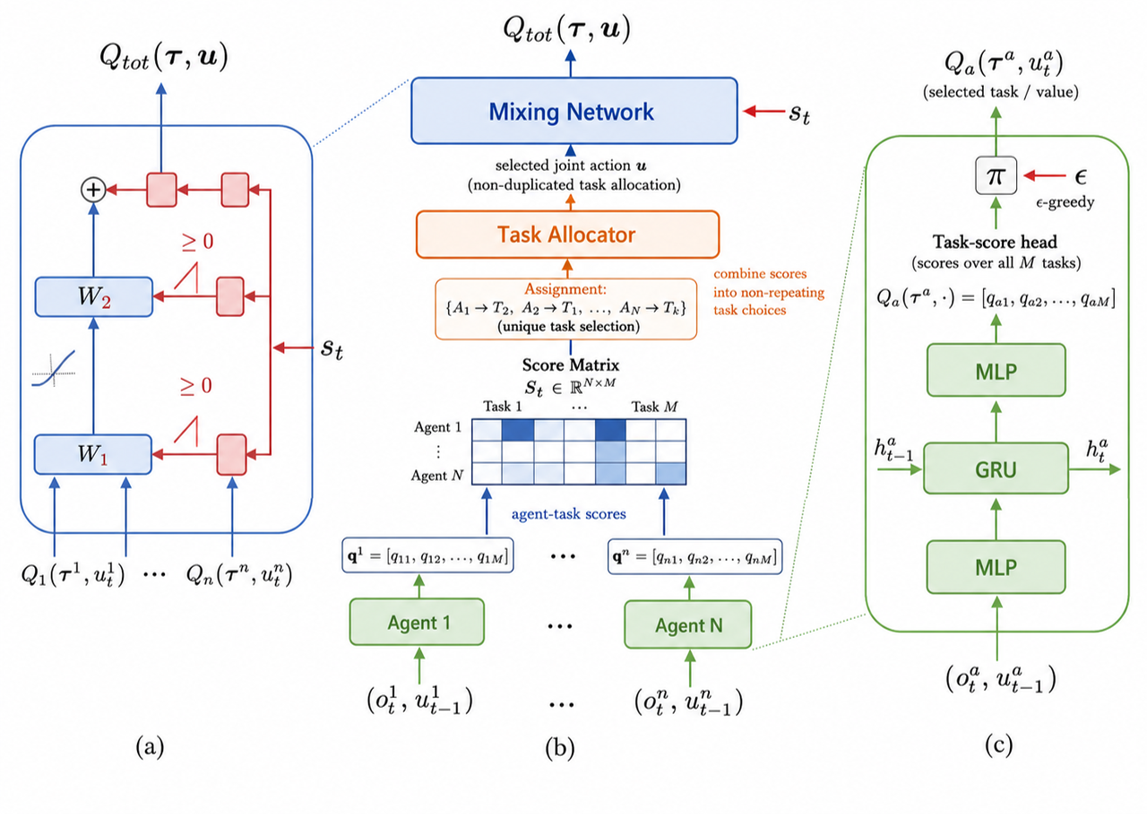
\includegraphics[width=0.92\linewidth]{../figure/task_allo.png}
\caption{Unique task assignment process in the platform. The scheduler receives visible orders and drone states, masks infeasible choices, and converts agent decisions into conflict-free executable assignments.}
\label{fig:task-allocation}
\end{figure*}

\begin{figure}[t]
\small
\begin{verbatim}
Algorithm 3 Unique task action selection
Input: agent Q-values, action masks
Output: conflict-free actions
1: mask unavailable actions
2: collect all feasible (agent, task, Q) triples
3: sort triples by Q in descending order
4: for each triple (i, a, Q) do
5:     if agent i and task a are both unused then
6:         assign action a to agent i
7:         mark i and a as used
8: assign NoOperation to unselected agents
9: return selected actions
\end{verbatim}
\caption{Unique task assignment pseudocode used by IQL-U, VDN-U, and QMIX-U.}
\label{fig:unique-pseudo}
\end{figure}

\section{Experimental Setup}

All algorithms are evaluated on the same shared environment and exported through the same comparison metric schema. The main environment settings are shown in Table~\ref{tab:setup}. Results are aggregated in the comparison directory of the platform and plotted with English metric labels.

\begin{table}[t]
\centering
\caption{Main simulation configuration.}
\label{tab:setup}
\begin{tabular}{ll}
\toprule
Item & Value \\
\midrule
Episode limit & 2000 steps \\
Number of drones & 10 \\
Number of generated tasks & 60 \\
Observable task slots & 8 \\
Charging stations & 10 \\
Task priorities & 1--3 \\
Task weights & 1--4 \\
Deadline offset & 200--300 steps \\
Drone carrying capacity & 5 weight units \\
Battery capacity & 15000 Wh \\
Drone speed & 200 simulation units \\
\bottomrule
\end{tabular}
\end{table}

The evaluation metrics include completion rate, timeout rate, average delay, average delay per priority level, generation-to-assignment waiting time, assignment-to-loading waiting time, loading-to-delivery time, average and maximum generation-to-completion time, and total energy consumption. The weighted overall score is a higher-is-better summary:
\begin{equation}
\begin{split}
S = &0.18C + 0.22(1-T) + 0.15(1-D) + 0.15(1-D_p)\\
&+ 0.14(1-G) + 0.16(1-E),
\end{split}
\end{equation}
where $C$ is completion rate, $T$ is timeout rate, $D$ is normalized average delay, $D_p$ is normalized priority-weighted delay, $G$ is normalized average generation-to-completion time, and $E$ is normalized energy consumption. Except for completion rate, lower raw values are better and are converted into capability scores by min-max normalization.

\begin{figure*}[t]
\centering
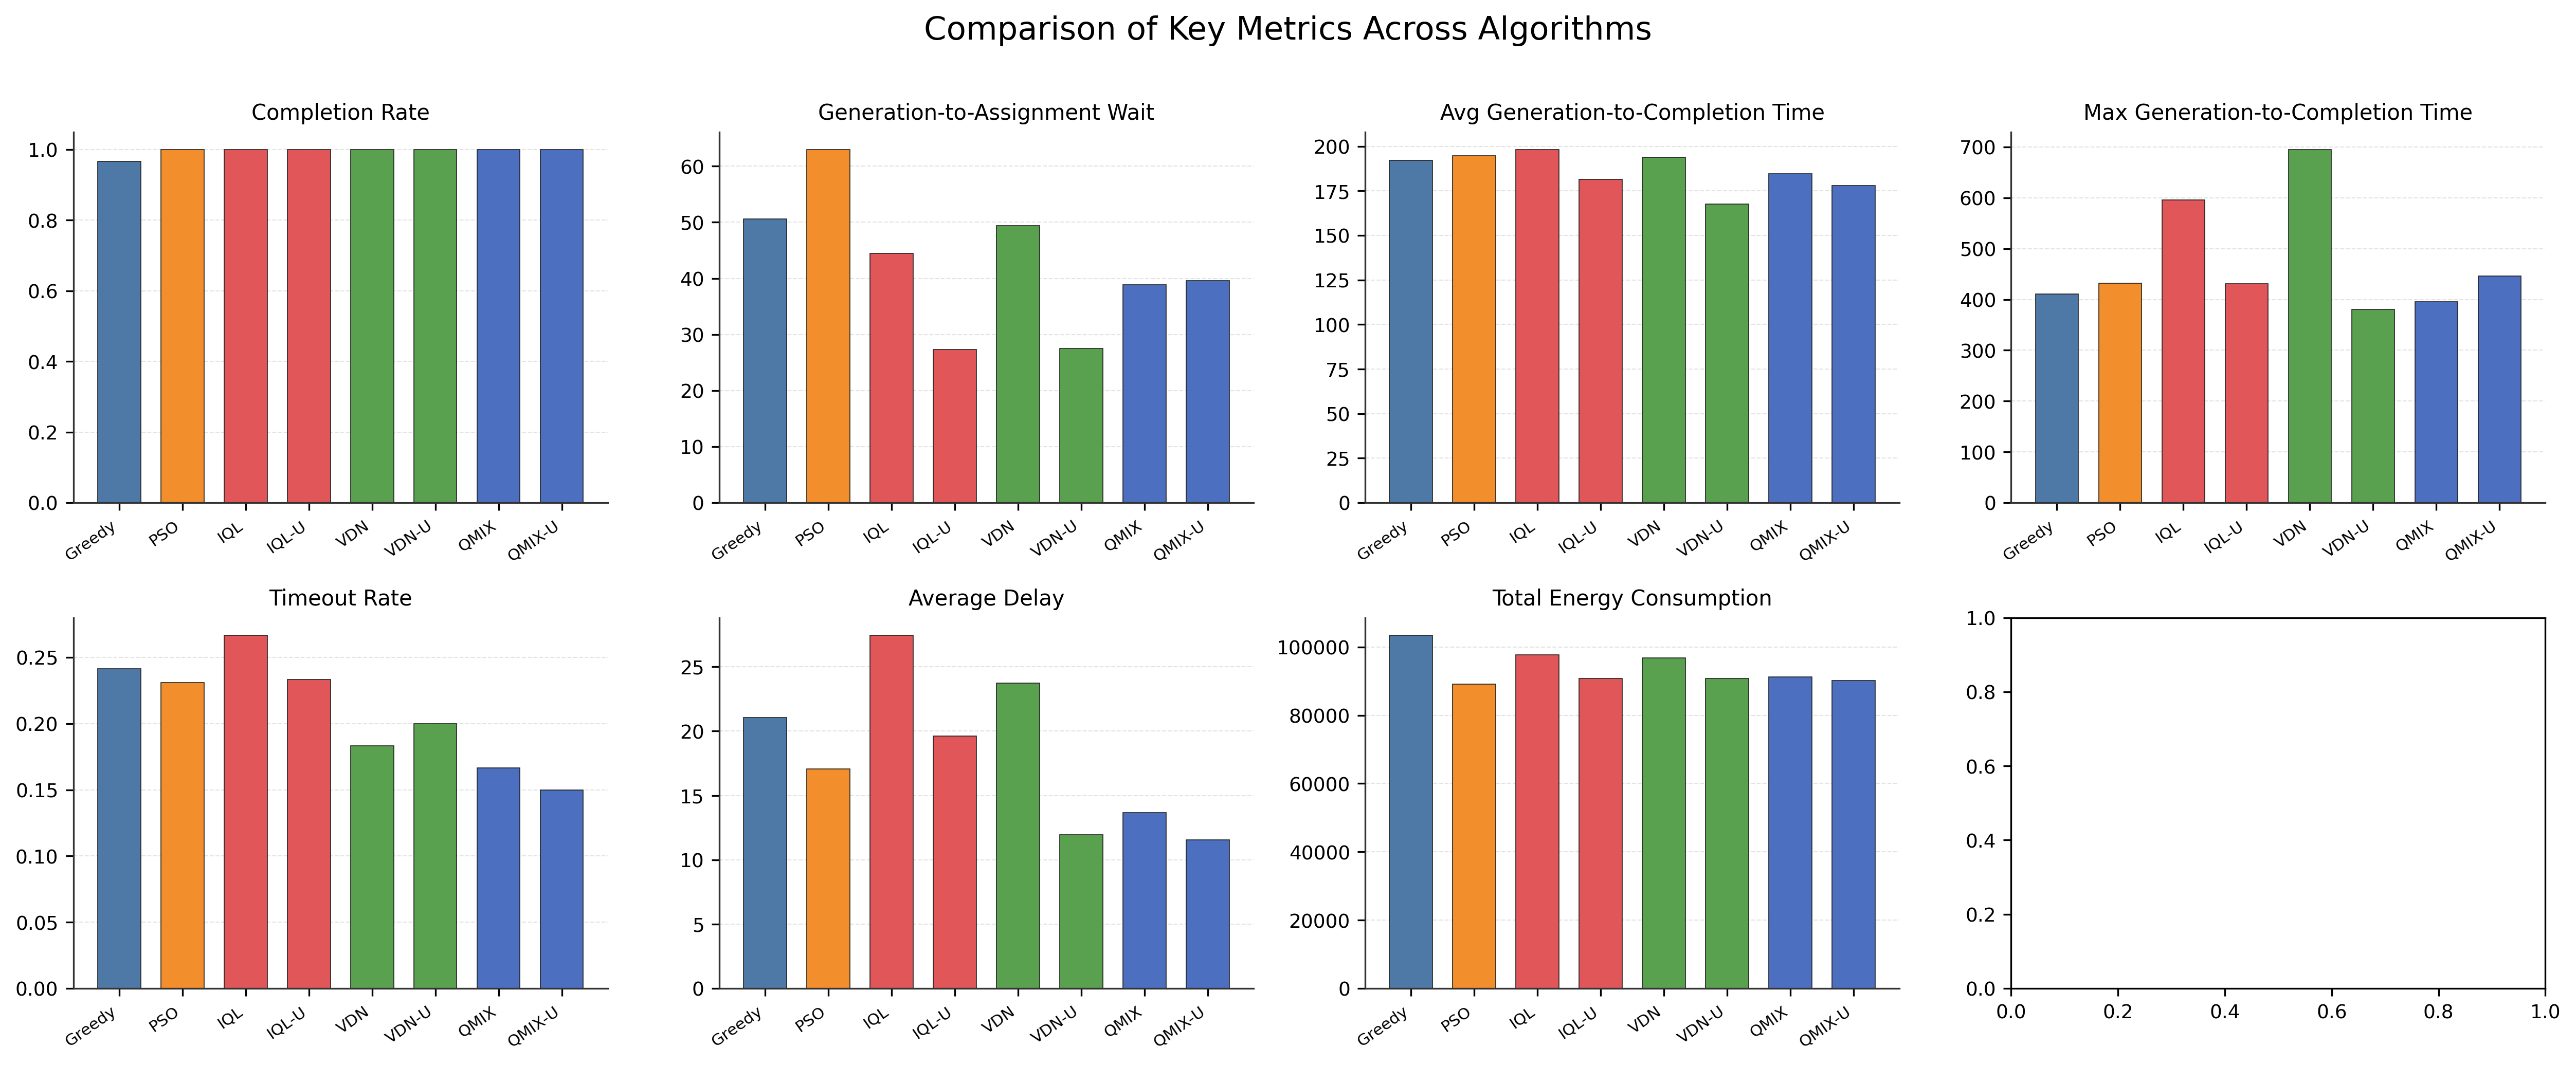
\includegraphics[width=0.95\linewidth]{../figure/bar_all_metrics_overview.png}
\caption{Overview of normalized and raw comparison indicators generated from the shared comparison pipeline.}
\label{fig:all-overview}
\end{figure*}

\section{Results and Analysis}

\subsection{Overall Comparison}

Table~\ref{tab:main-results} summarizes the main results. Greedy completes 58 of 60 tasks, while all other methods complete all 60 generated tasks. Among the learning methods, QMIX-U has the lowest timeout rate and the best weighted overall score. VDN-U has the shortest average generation-to-completion time and very low average delay. PSO provides a strong non-learning baseline with full completion and lower energy consumption than greedy.

\begin{figure*}[t]
\centering
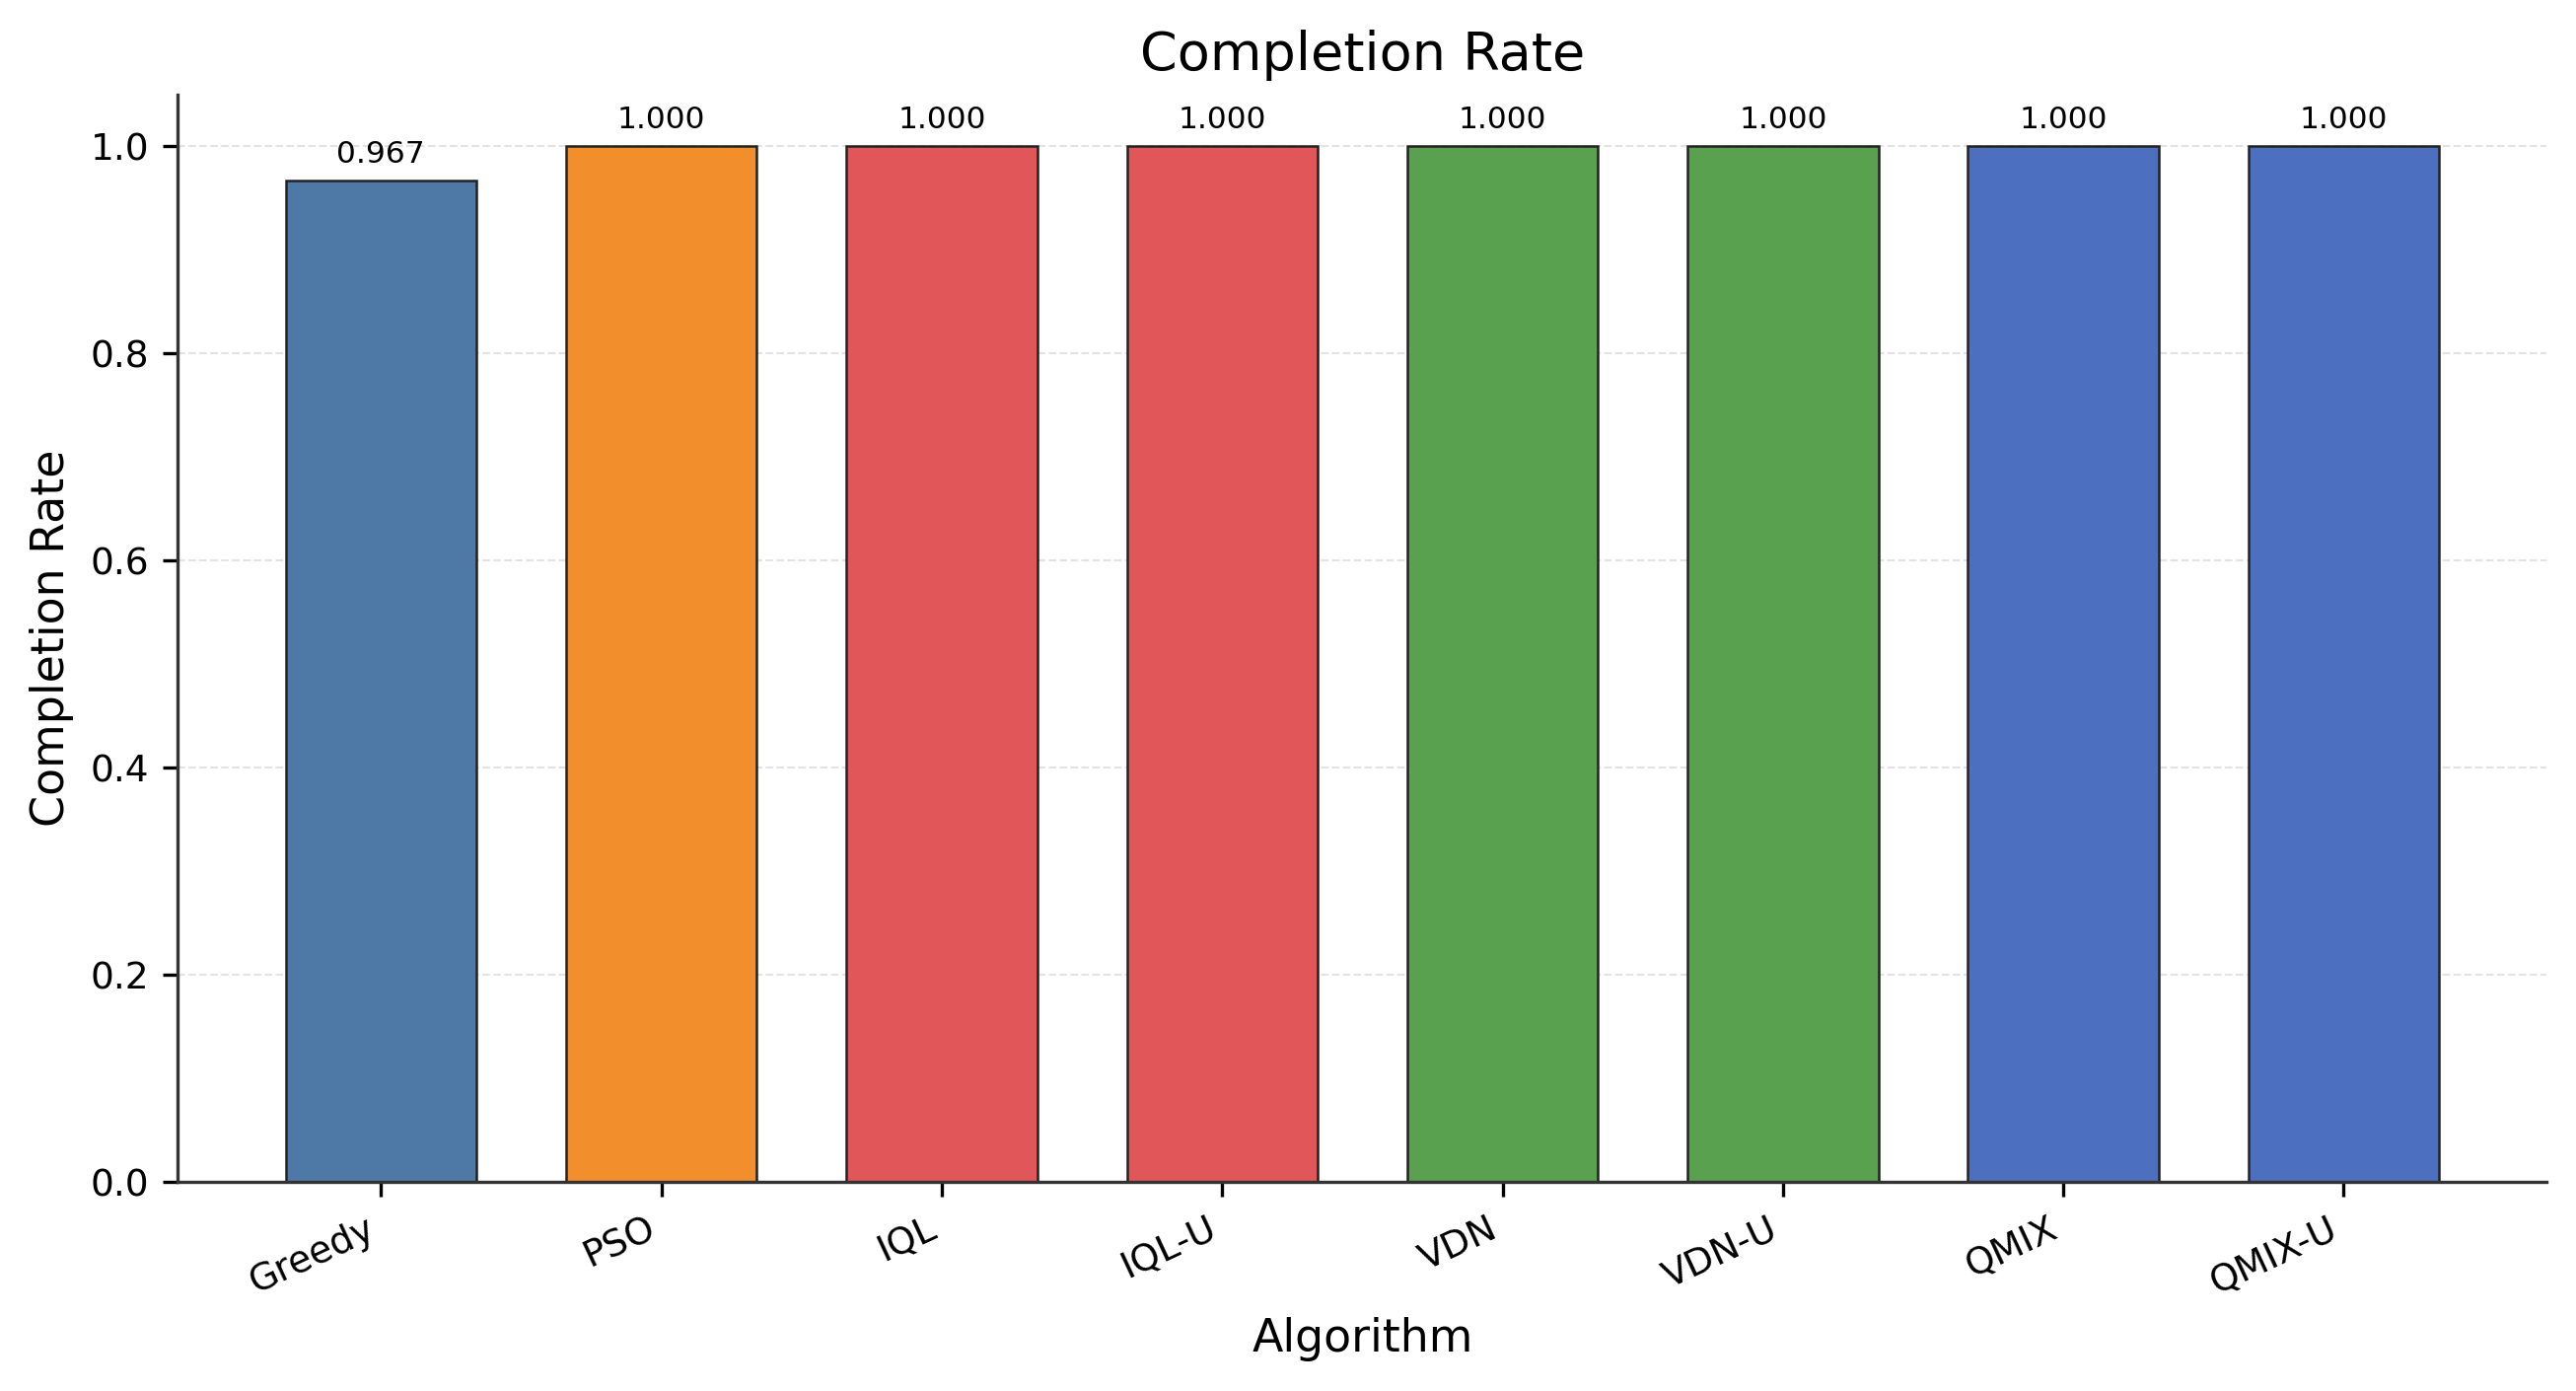
\includegraphics[width=0.48\linewidth]{../figure/bar_completion_rate.png}
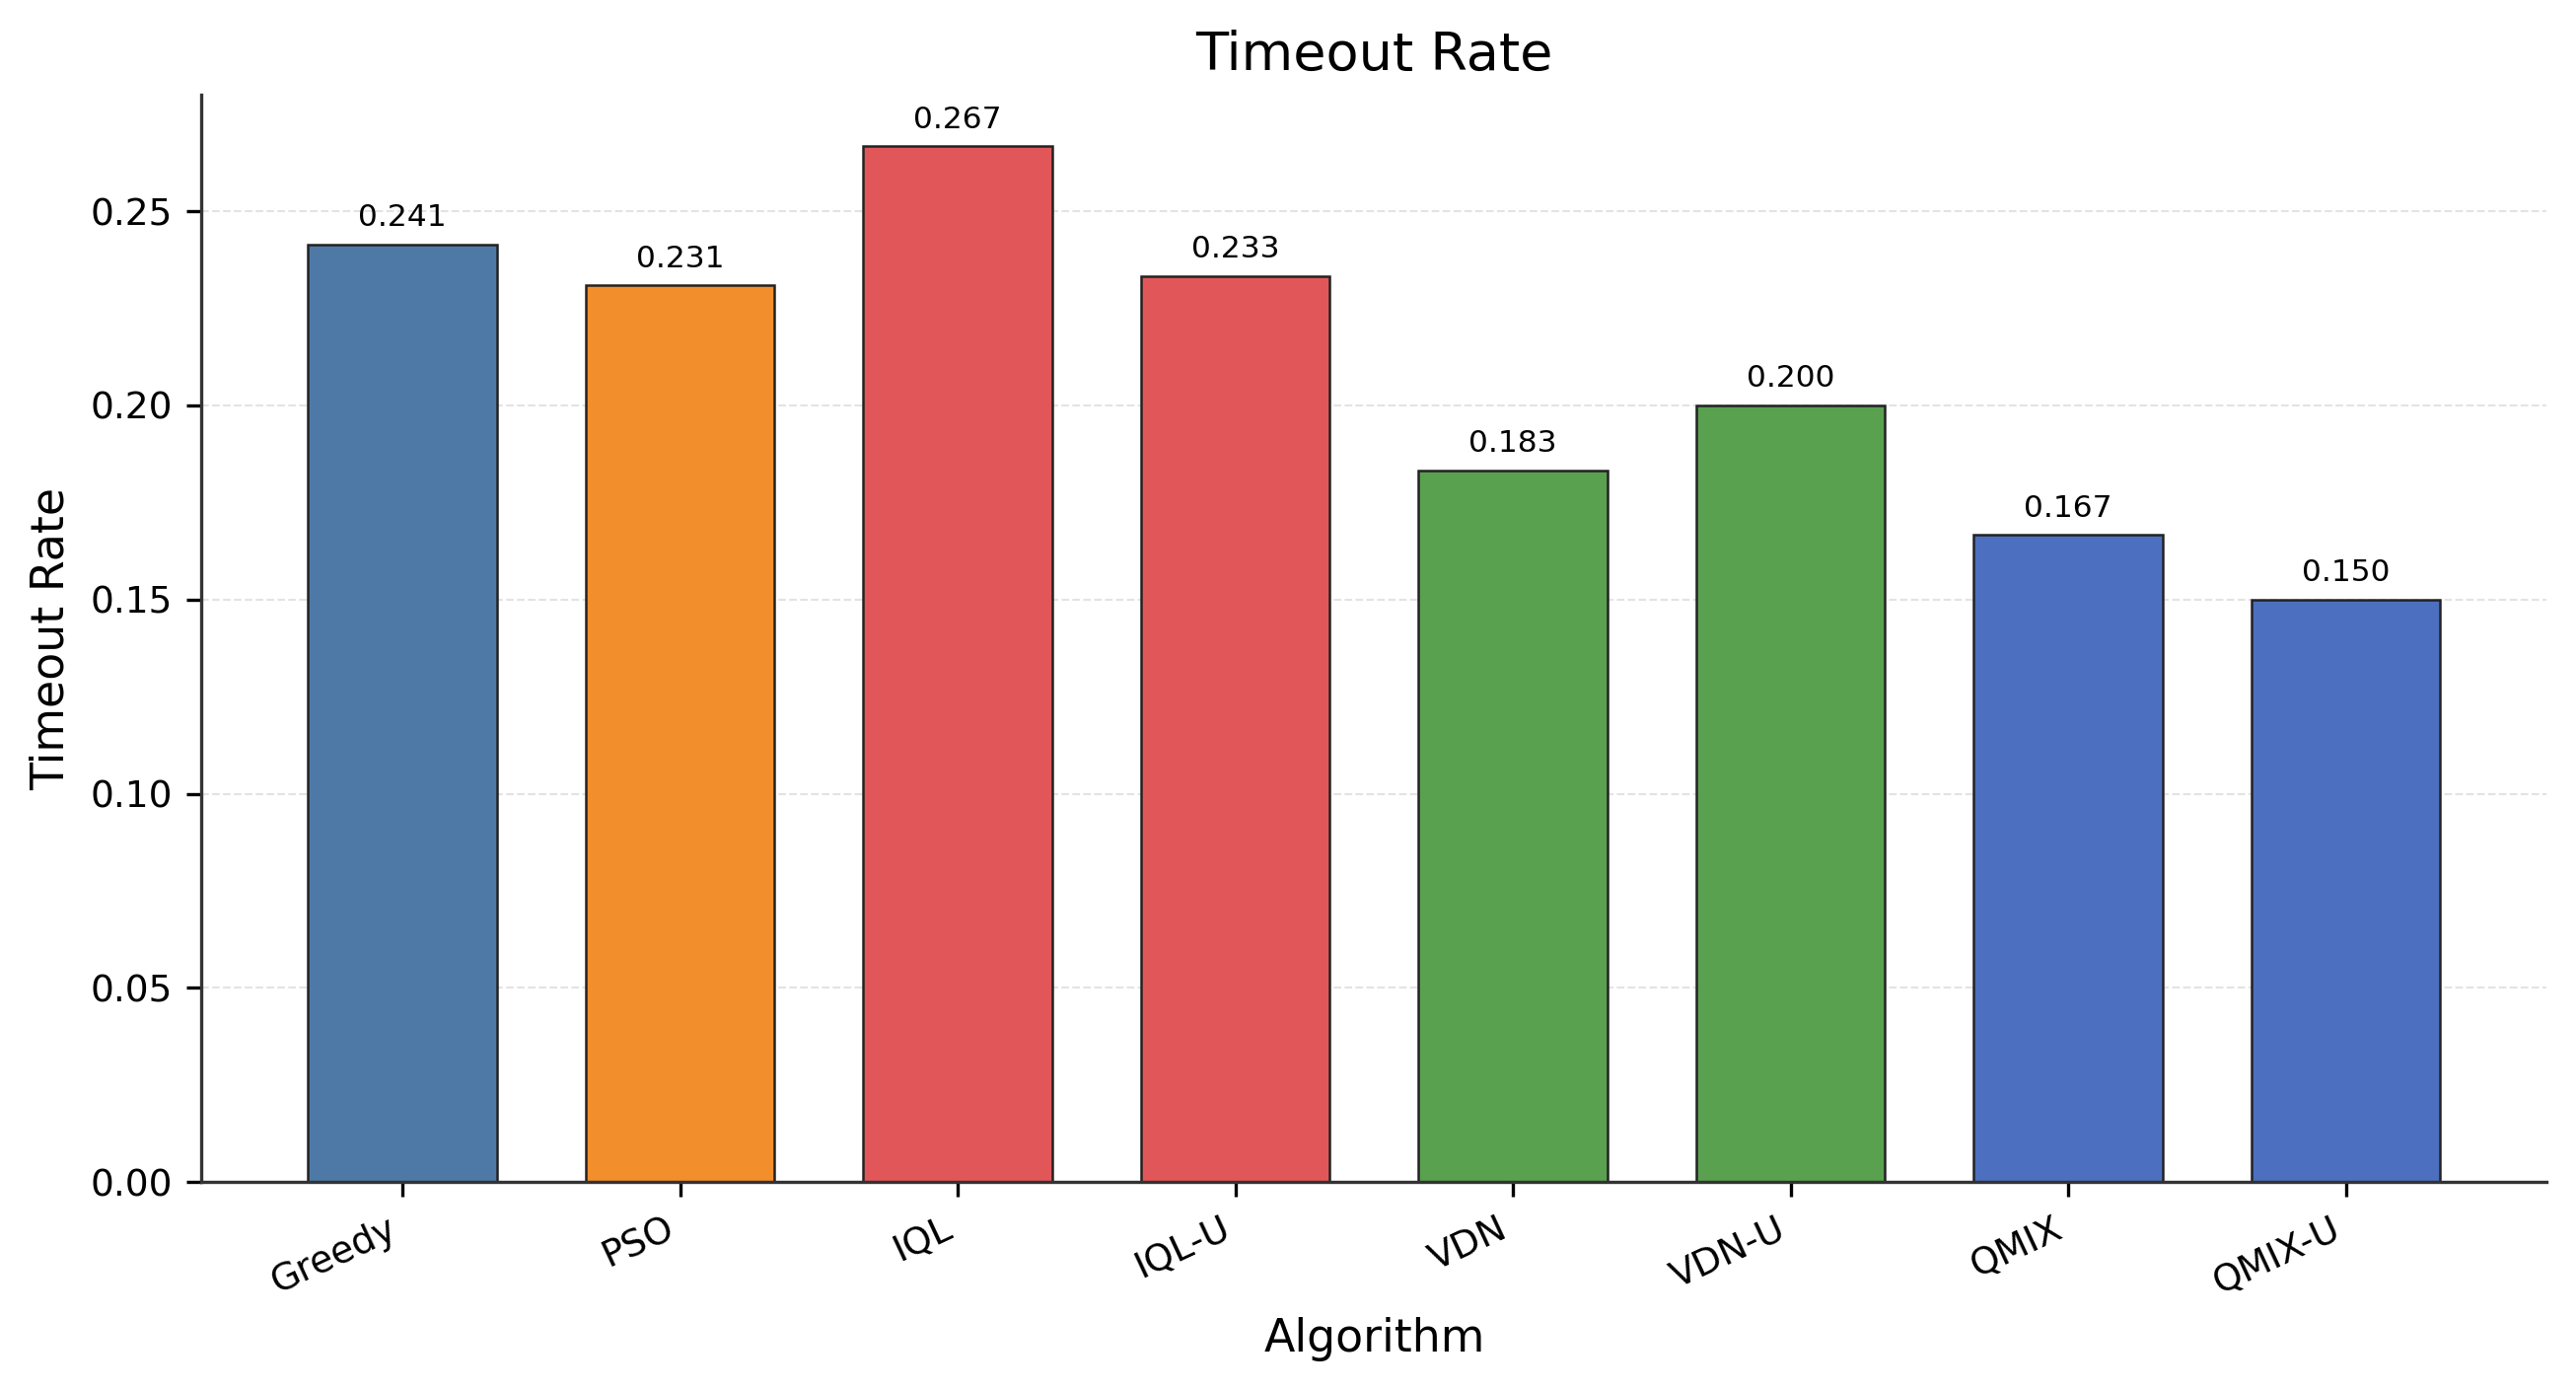
\includegraphics[width=0.48\linewidth]{../figure/bar_timeout_rate.png}
\caption{Completion rate and timeout rate comparison.}
\label{fig:completion-timeout}
\end{figure*}

\begin{table*}[t]
\centering
\caption{Comparison of scheduling algorithms. Lower is better except for completion rate and weighted score.}
\label{tab:main-results}
\begin{tabular}{lrrrrrrr}
\toprule
Algorithm & Completion & Timeout & Avg. delay & Avg. completion & Max completion & Energy & Score \\
\midrule
Greedy & 0.967 & 0.241 & 21.07 & 192.22 & 411.0 & 103415.8 & 0.371 \\
PSO & 1.000 & 0.231 & 17.05 & 194.72 & 432.1 & 89177.6 & 0.616 \\
IQL & 1.000 & 0.267 & 27.45 & 198.18 & 596.0 & 97632.2 & 0.245 \\
IQL-U & 1.000 & 0.233 & 19.63 & 181.55 & 431.0 & 90733.8 & 0.625 \\
VDN & 1.000 & 0.183 & 23.75 & 193.73 & 695.0 & 96823.4 & 0.470 \\
VDN-U & 1.000 & 0.200 & 11.93 & 167.52 & 380.0 & 90823.9 & 0.884 \\
QMIX & 1.000 & 0.167 & 13.67 & 184.75 & 396.0 & 91288.6 & 0.814 \\
QMIX-U & 1.000 & 0.150 & 11.55 & 177.92 & 446.0 & 90107.1 & 0.929 \\
\bottomrule
\end{tabular}
\end{table*}

\subsection{Effect of Unique Task Assignment}

The unique-task-assignment variants consistently improve IQL and QMIX, and strongly improve VDN in the weighted score. IQL-U reduces average generation-to-assignment wait from 44.42 to 27.32 and reduces average delay from 27.45 to 19.63. VDN-U reduces average delay from 23.75 to 11.93 and average generation-to-completion time from 193.73 to 167.52. QMIX-U further reduces timeout rate from 0.167 to 0.150 and average delay from 13.67 to 11.55.

These results support the design motivation of the task assignment mechanism. When multiple agents select tasks independently, duplicate choices and invalid actions waste decision opportunities. Enforcing uniqueness makes the joint action more feasible and reduces the noise introduced by conflicts. This is particularly useful in a logistics setting where each order can only be served by one drone.

\begin{figure*}[t]
\centering
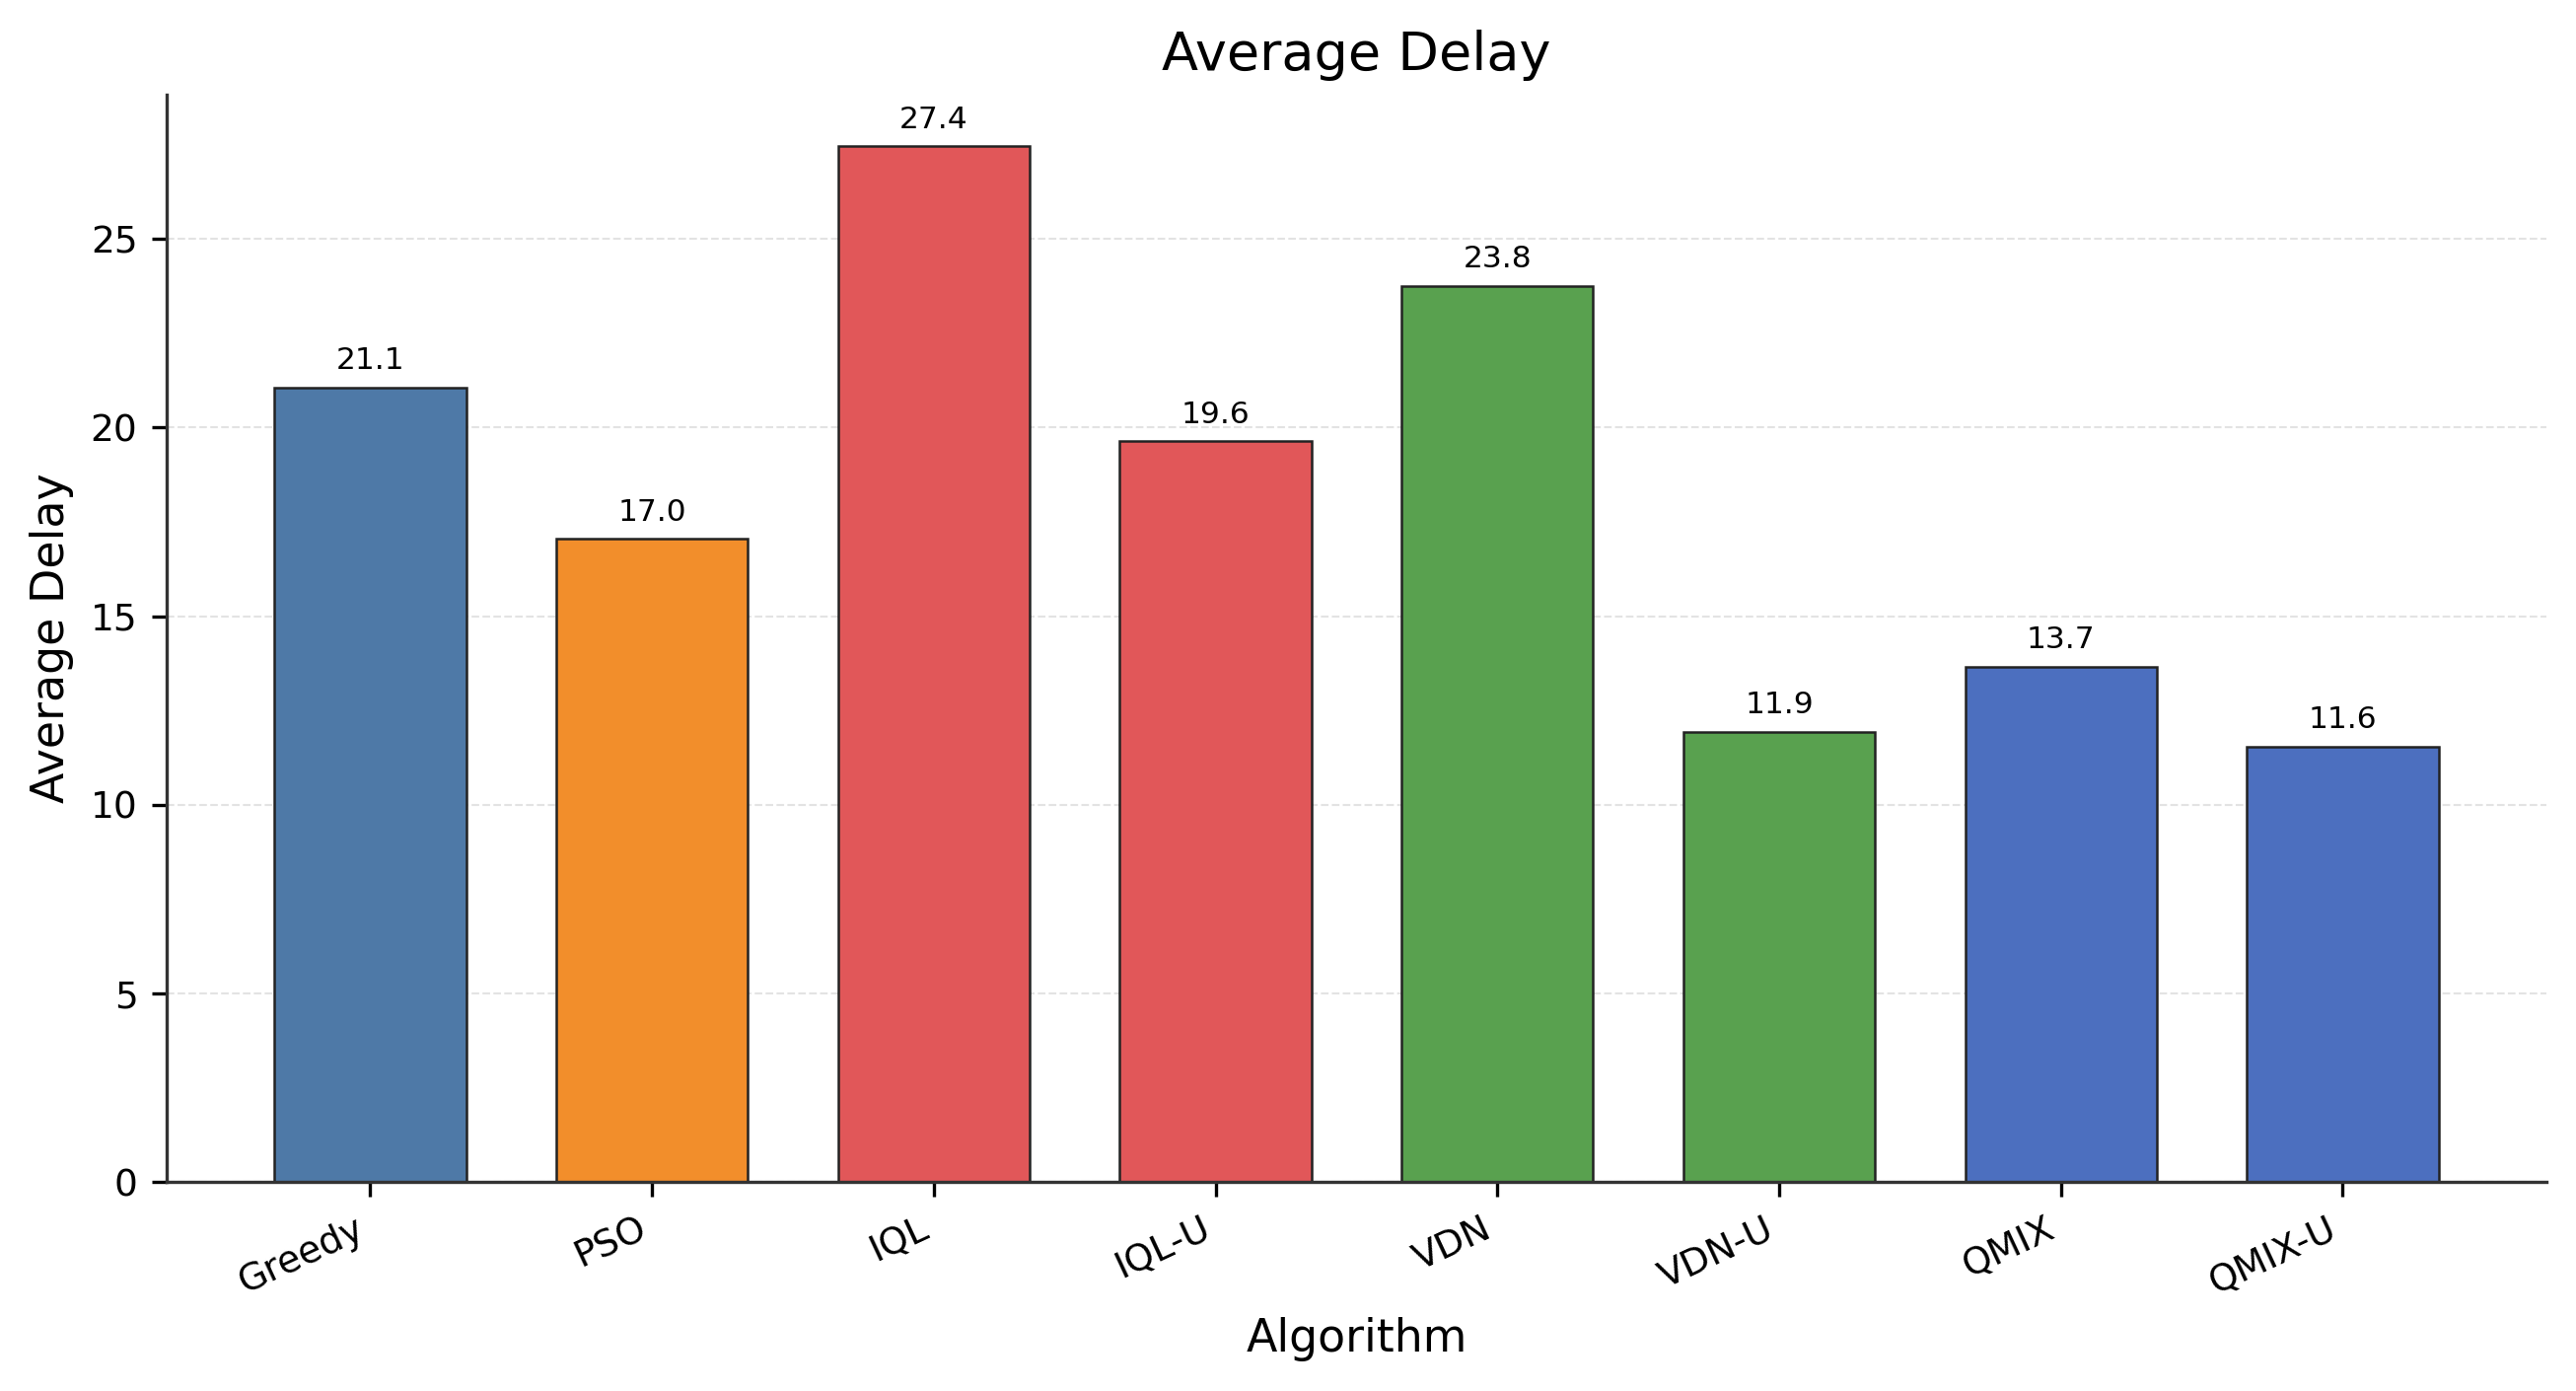
\includegraphics[width=0.48\linewidth]{../figure/bar_average_delay.png}
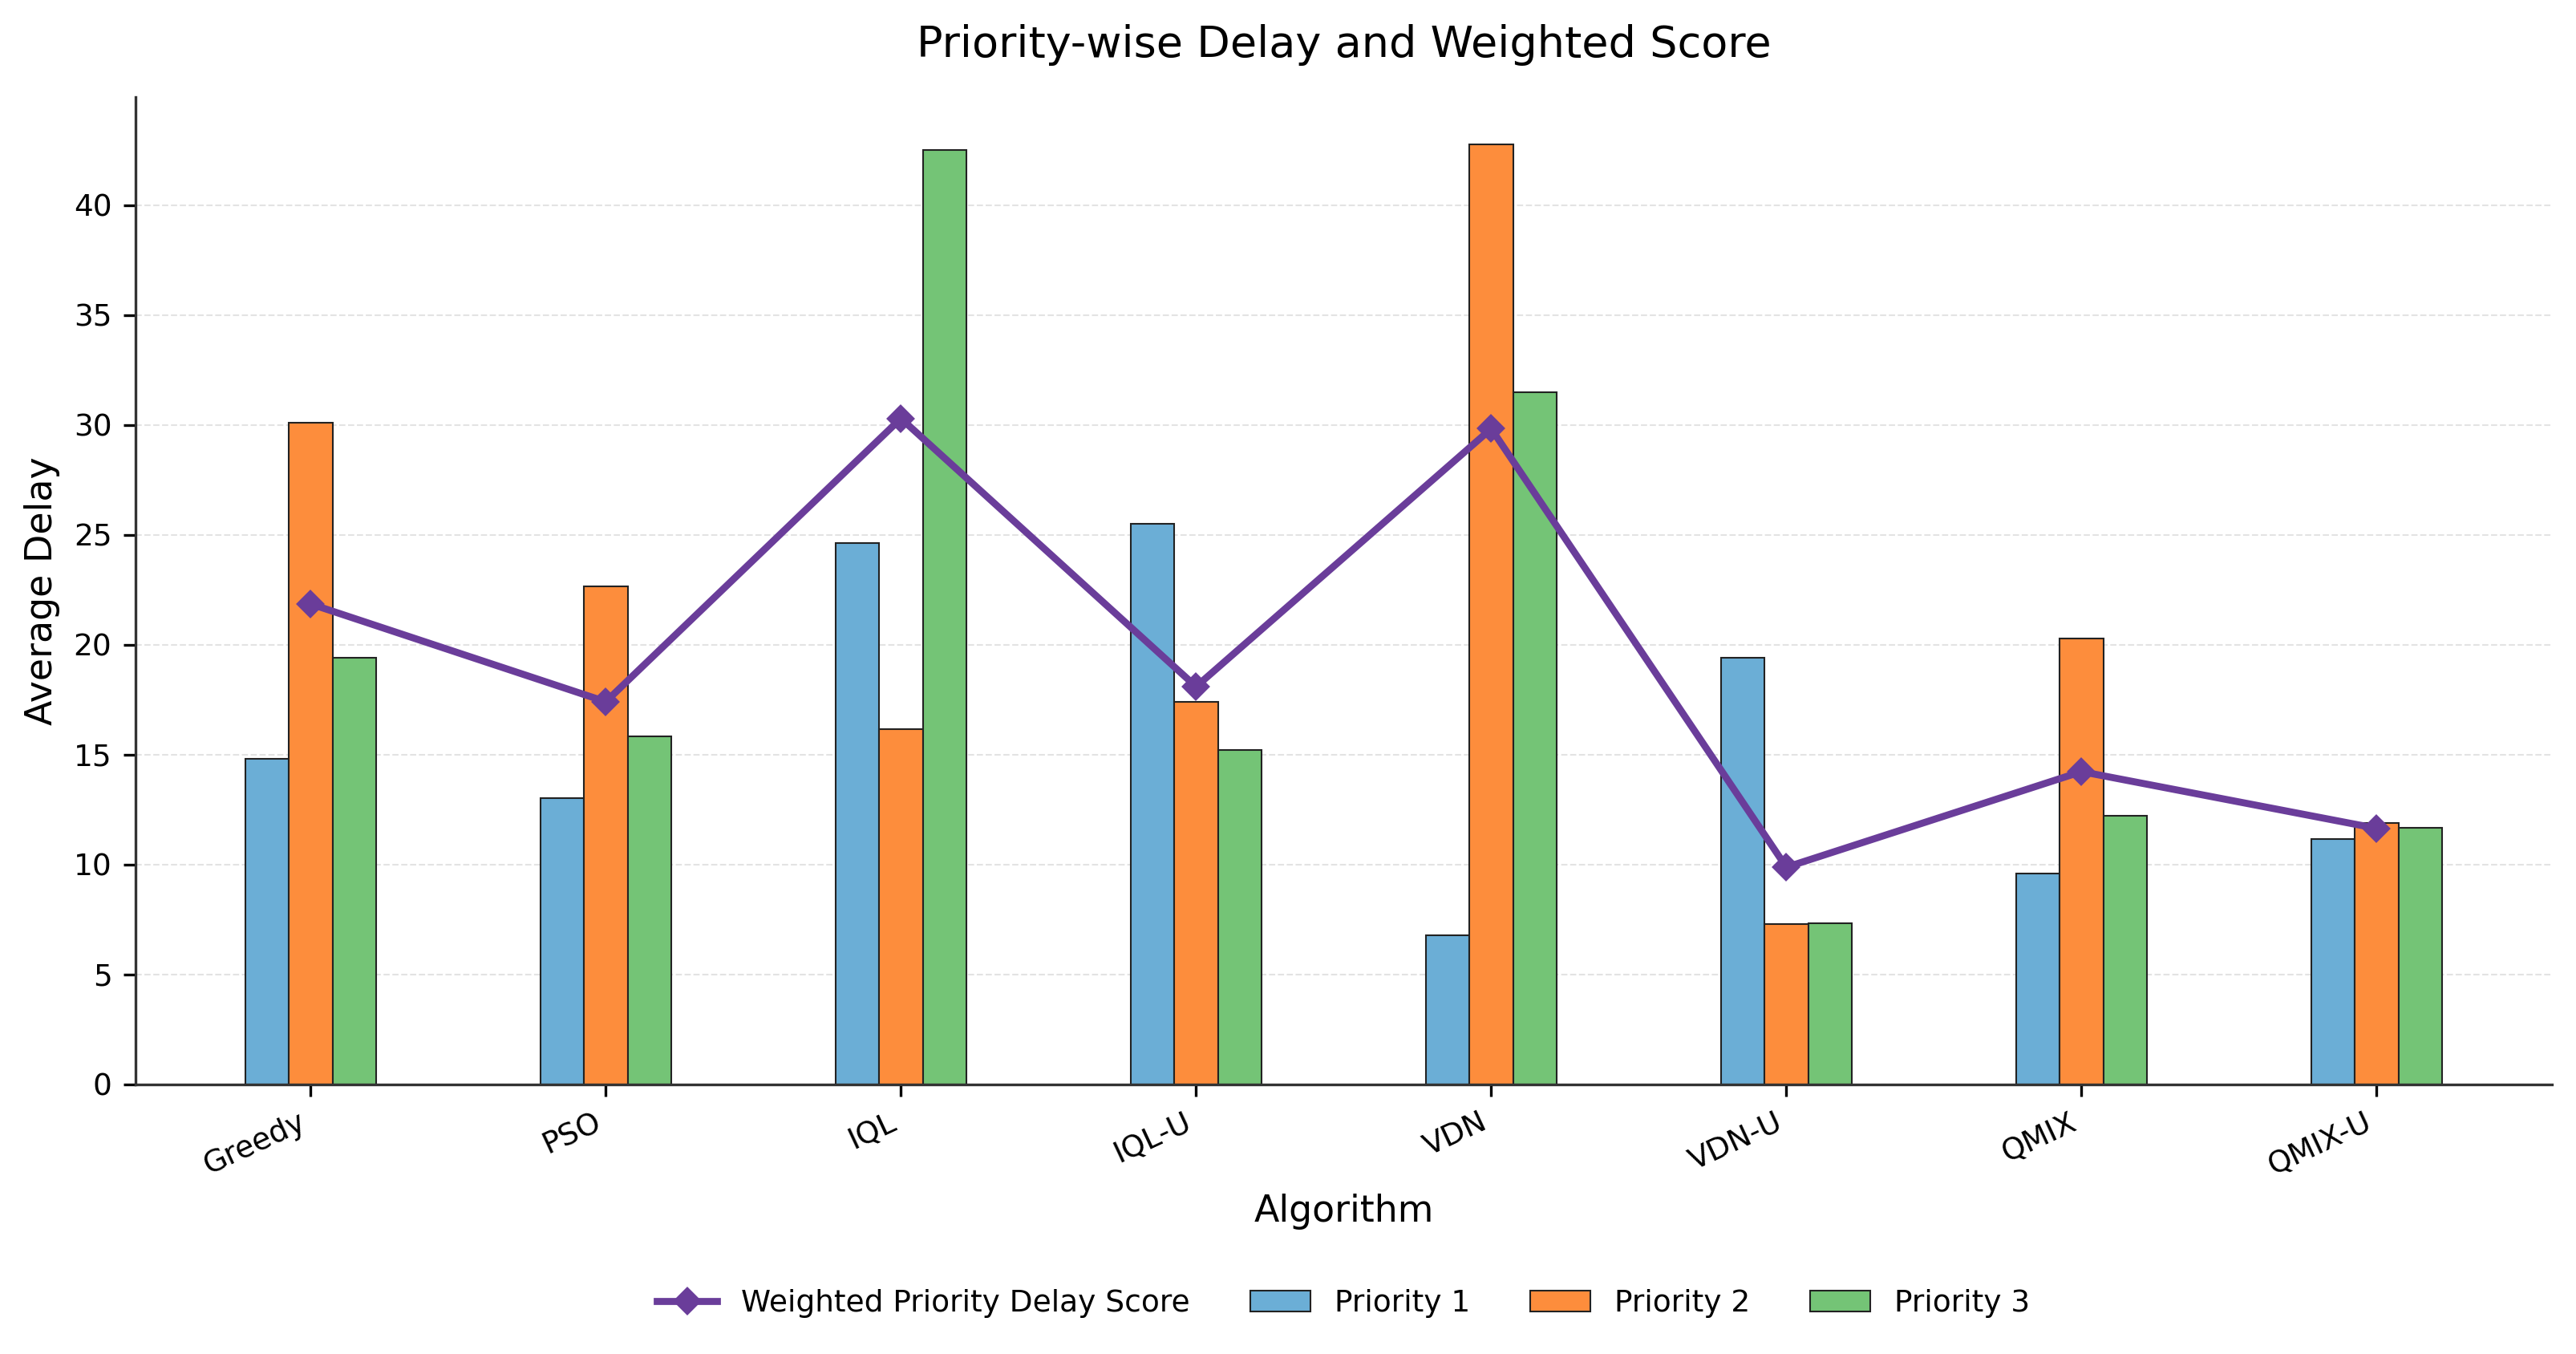
\includegraphics[width=0.48\linewidth]{../figure/bar_priority_delay_grouped.png}
\caption{Average delay and priority-wise delay comparison.}
\label{fig:delay}
\end{figure*}

\subsection{Heuristic and Swarm Intelligence Baselines}

The greedy scheduler is competitive on maximum completion time but has the only incomplete run and the highest total energy consumption. Its local-distance objective does not directly account for global workload balance or priority delay. PSO reaches full completion and the lowest total energy consumption in the table. This indicates that batch optimization over buffered tasks can produce energy-efficient assignments. However, PSO does not outperform the best MARL variants on timeout rate or weighted score, suggesting that learned policies can better adapt to dynamic order states when conflict handling is improved.

\begin{figure*}[t]
\centering
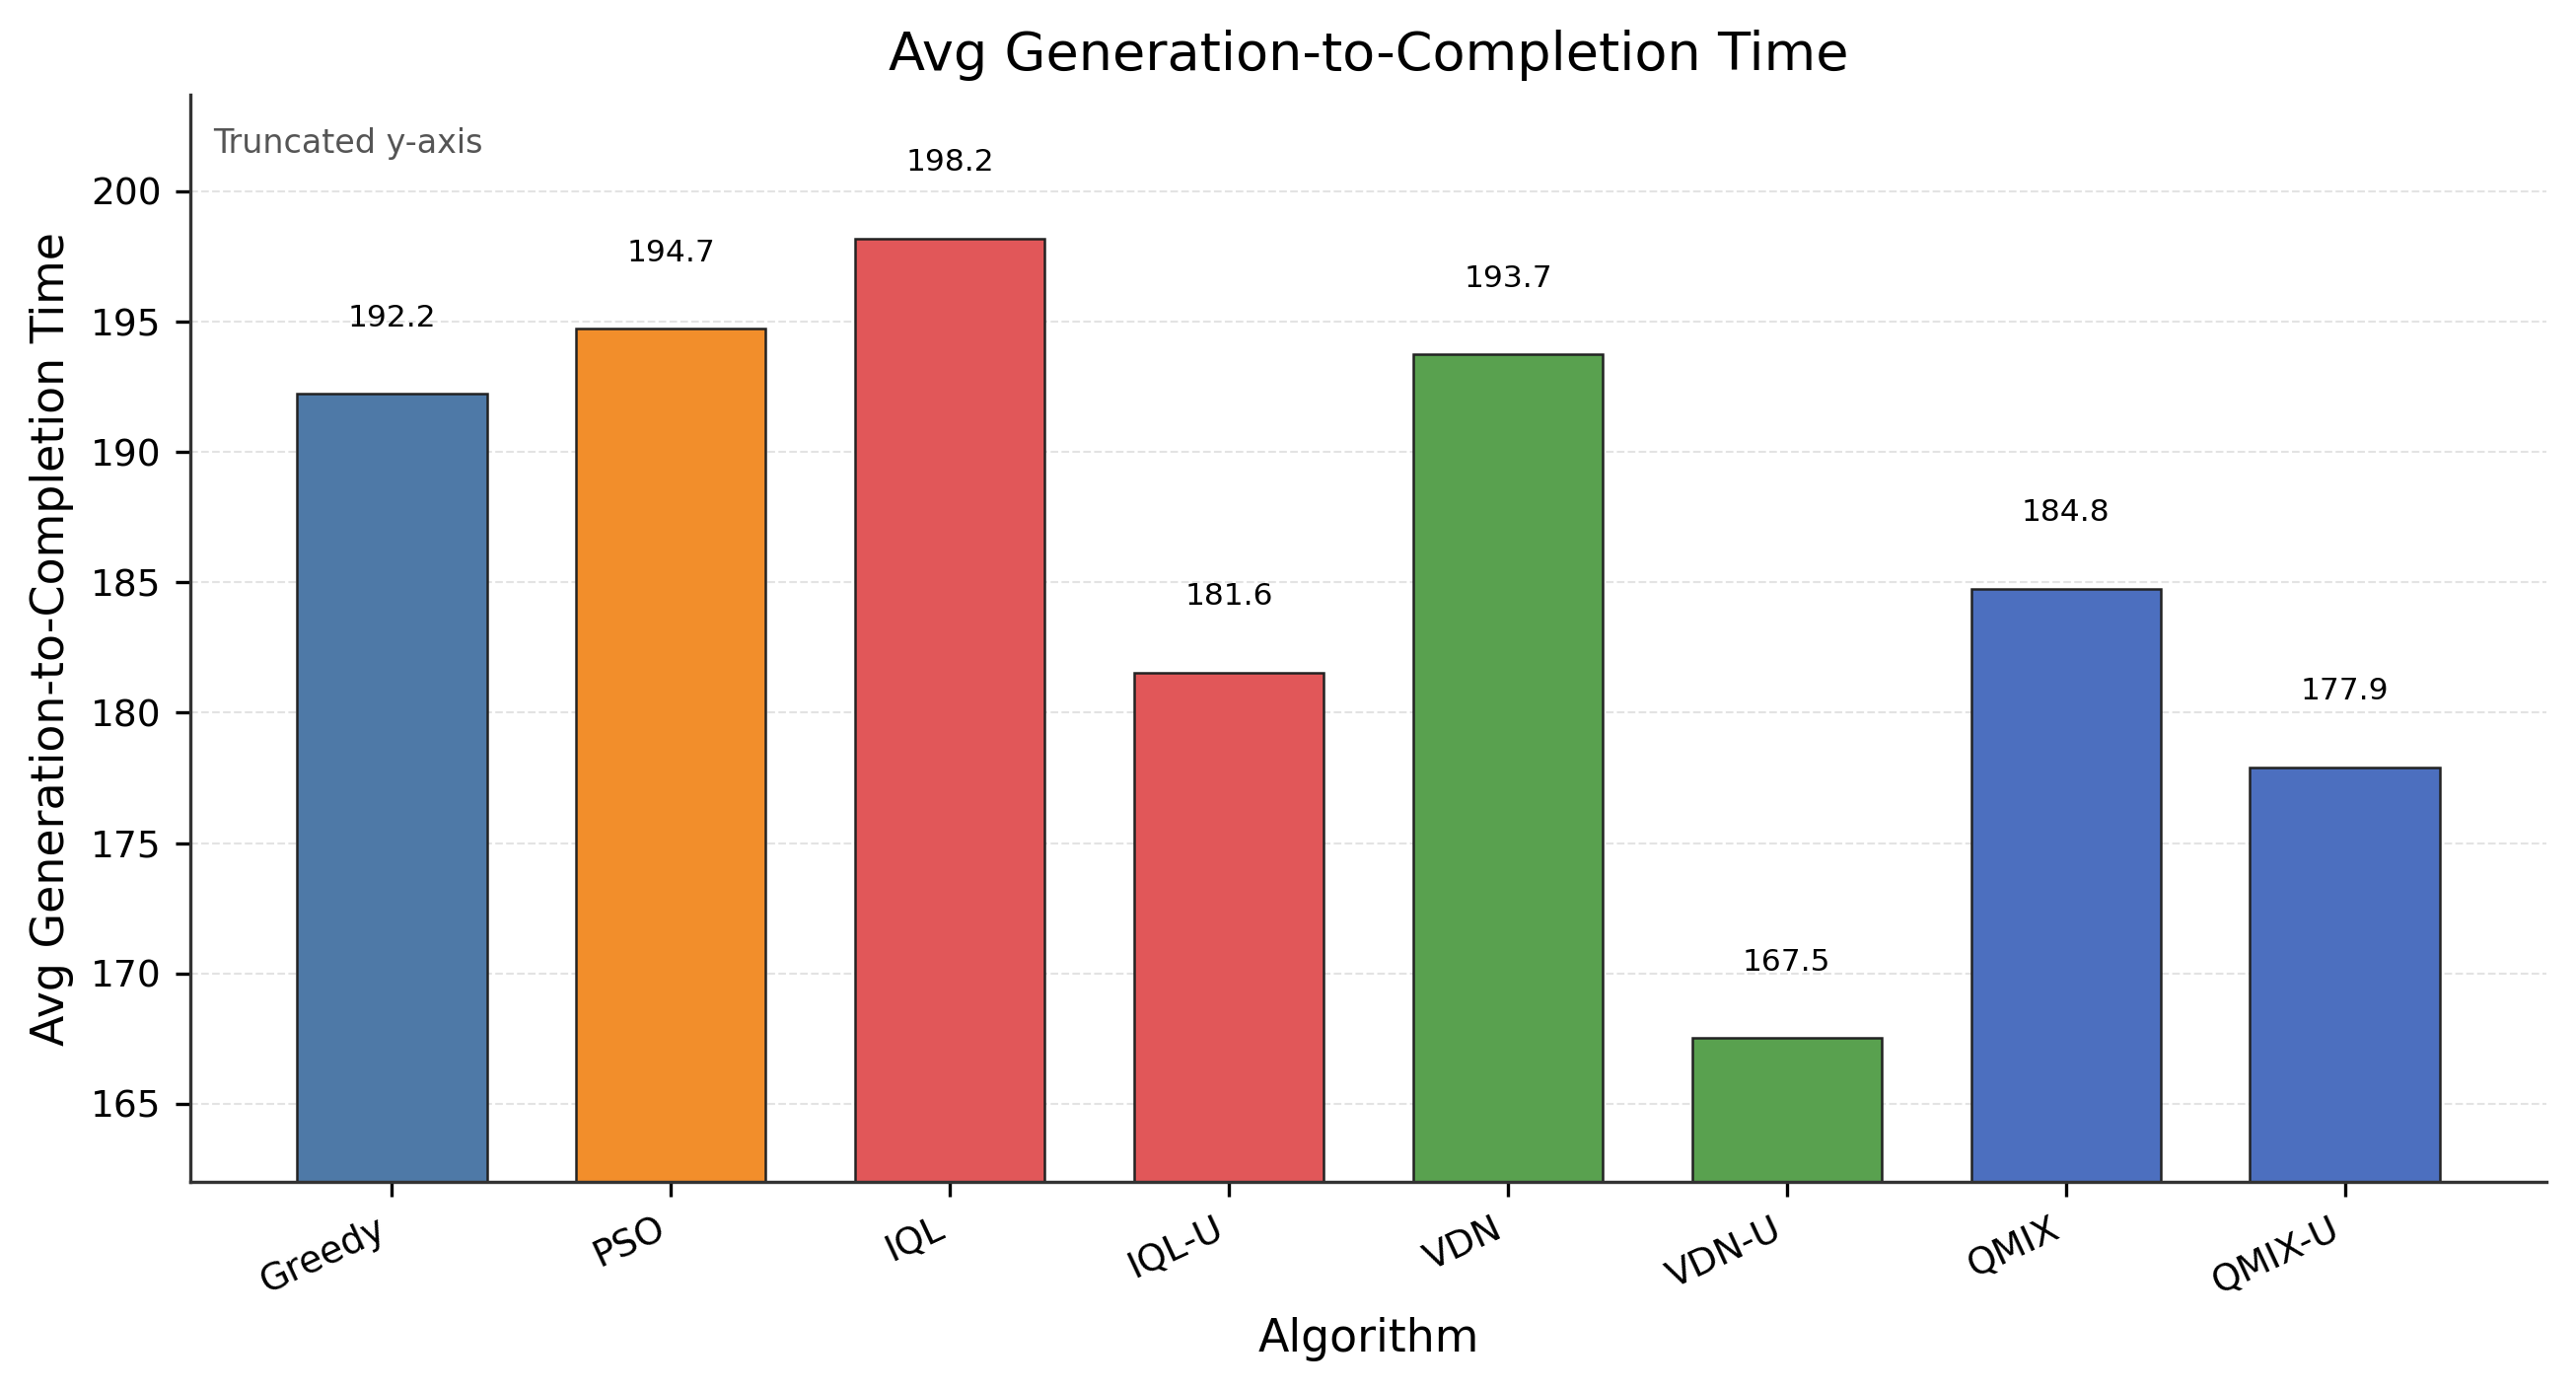
\includegraphics[width=0.48\linewidth]{../figure/bar_avg_generation_to_completion_time.png}
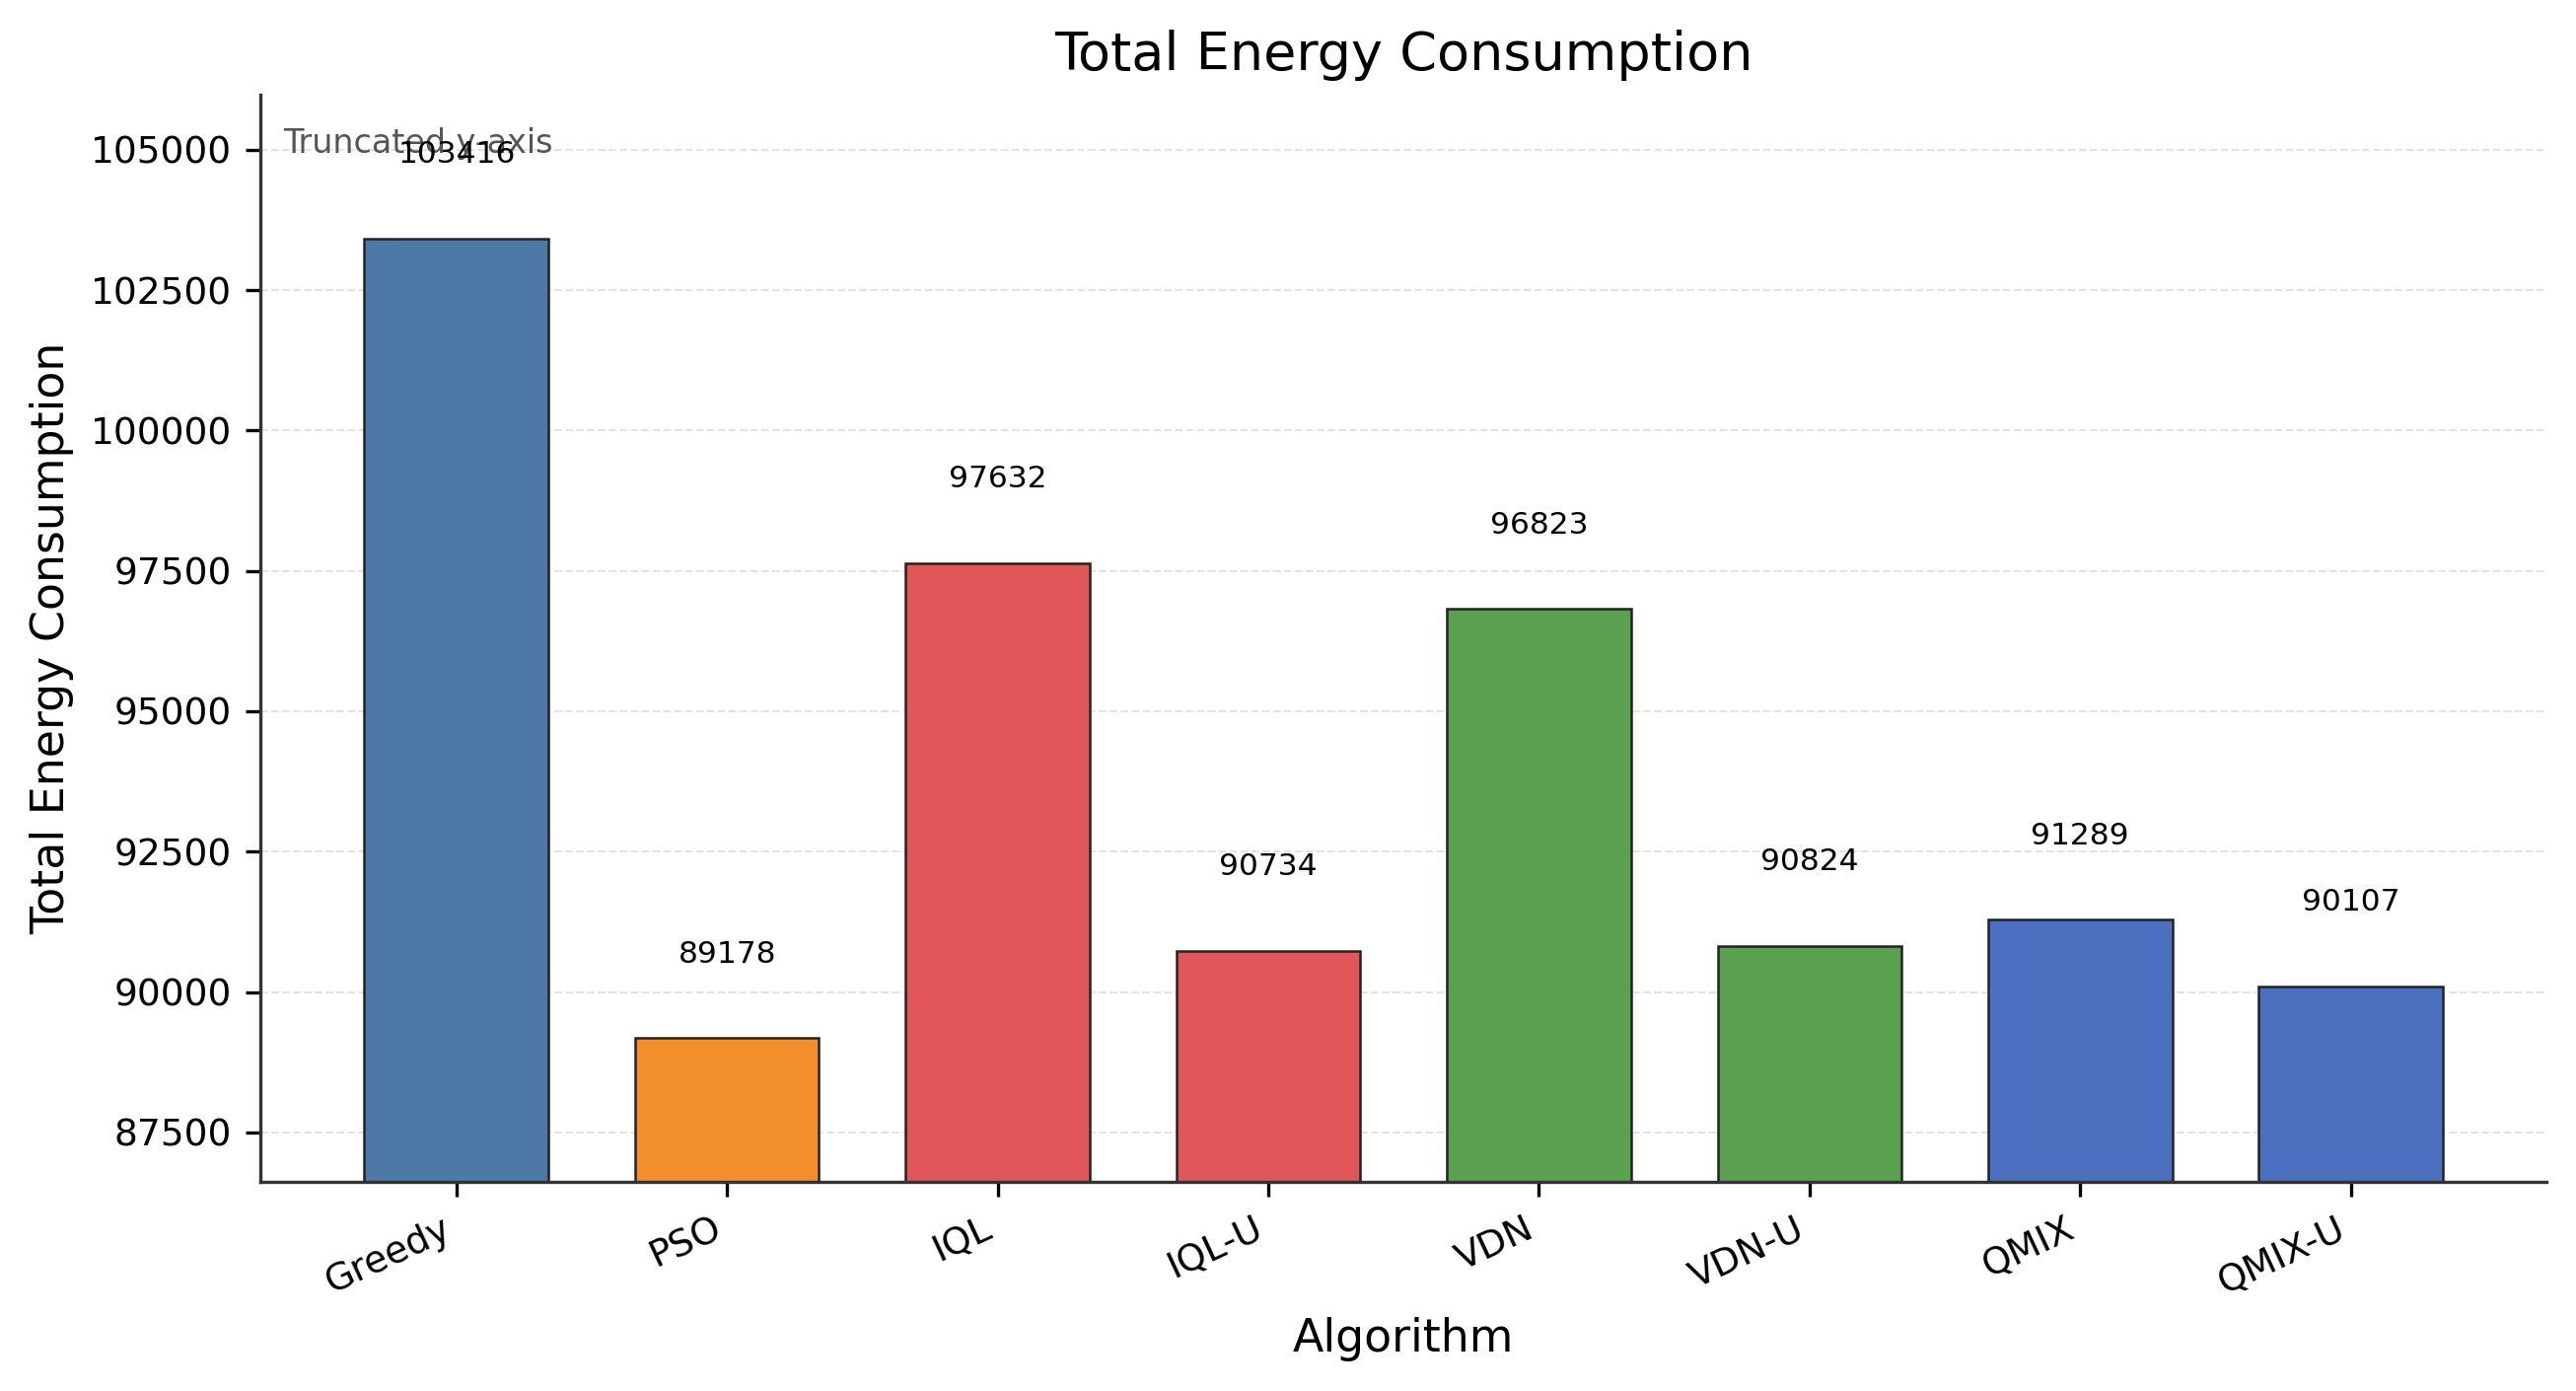
\includegraphics[width=0.48\linewidth]{../figure/bar_total_energy_consumption.png}
\caption{Average completion time and total energy consumption.}
\label{fig:time-energy}
\end{figure*}

\subsection{Best Performing Policy}

According to the weighted overall score, the ranking is QMIX-U, VDN-U, QMIX, IQL-U, PSO, VDN, Greedy, and IQL. The top methods are not simply those with full completion, since seven methods complete all tasks. The score rewards lower timeout, lower delay, shorter completion time, and lower energy consumption after normalization. QMIX-U performs best because it combines full completion, the lowest timeout rate, the lowest average delay, and competitive energy consumption.

\begin{figure}[t]
\centering
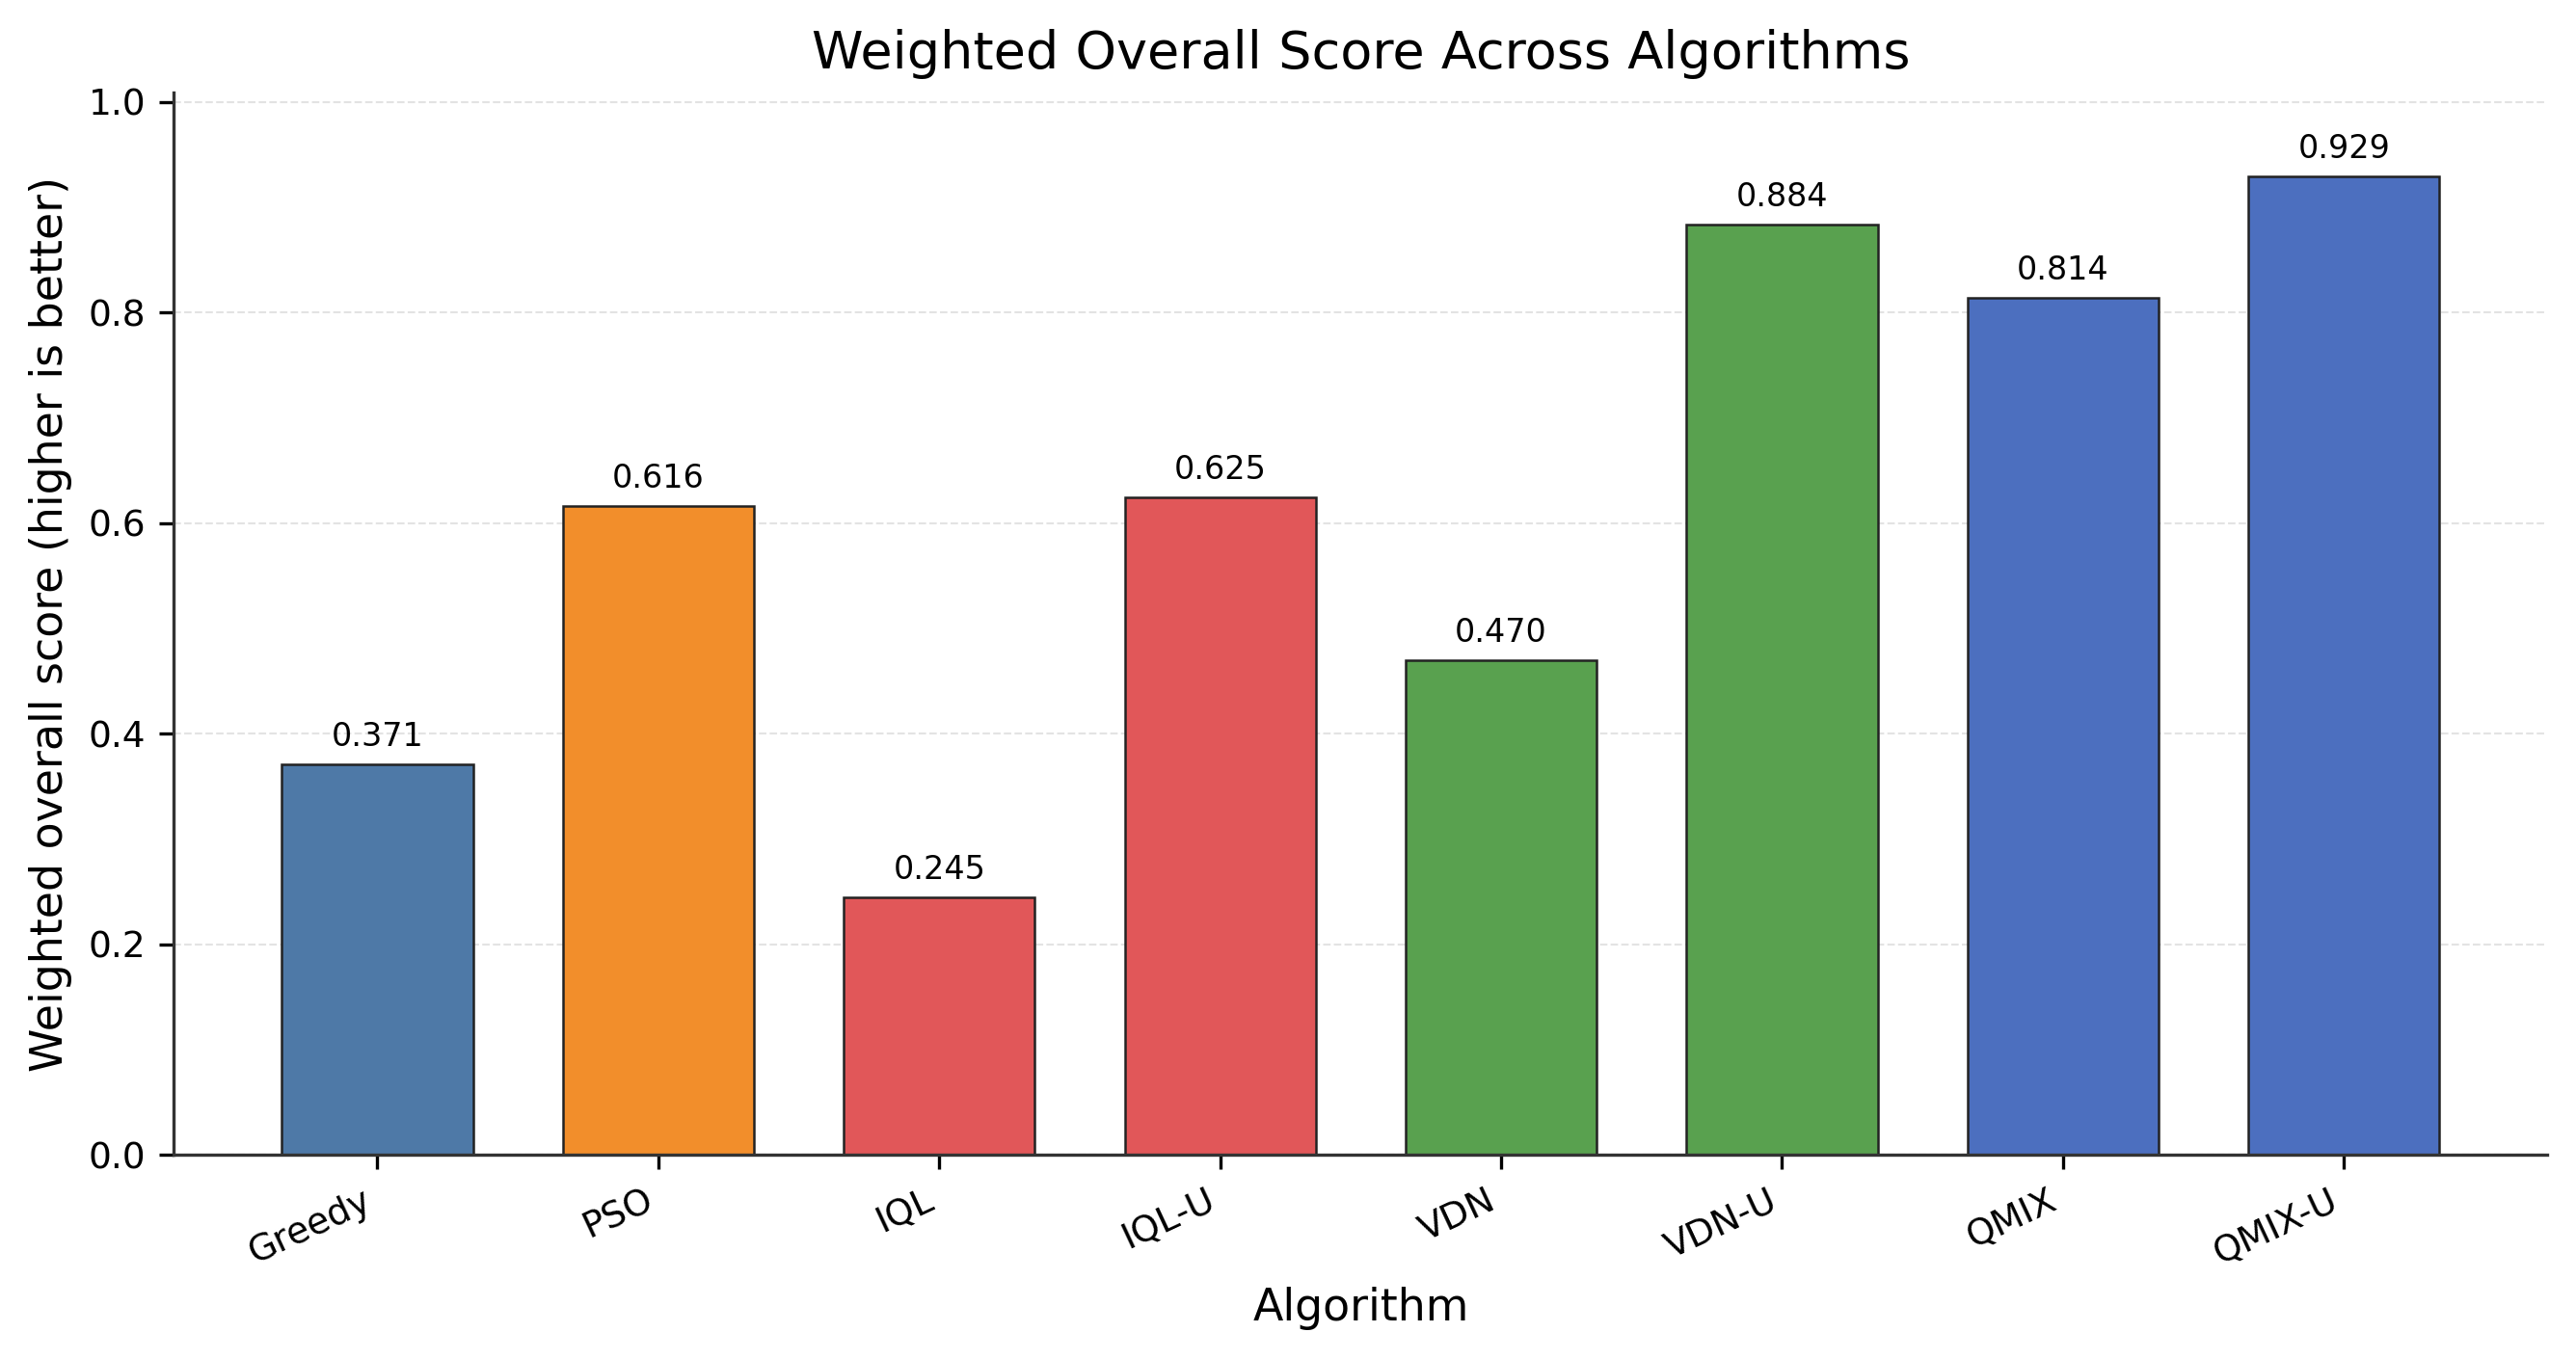
\includegraphics[width=\linewidth]{../figure/bar_weighted_overall_score.png}
\caption{Weighted overall score of all evaluated algorithms.}
\label{fig:score}
\end{figure}

\section{Discussion}

The comparison shows that algorithmic quality depends on both decision model and action feasibility. Greedy is simple and robust but lacks look-ahead. PSO improves global allocation through batch optimization and explicit multi-objective fitness. MARL policies can exploit richer state information, but their raw action formulation may violate mutual exclusion among tasks. The unique task assignment mechanism is therefore important: it does not change the logistics objective, but it changes the action execution layer so that learning signals correspond more closely to feasible dispatching decisions.

There are also limitations. The current experiment uses a fixed task scale and a fixed map configuration. More comprehensive validation should vary order density, drone count, charging station capacity, task priority distribution, and obstacle layout. The current weighted score is useful for presentation and comparison, but different applications may prefer different trade-offs between timeliness and energy. Future work can include adaptive weight selection, online retraining, stochastic travel times, and larger-scale experiments.

\section{Conclusion}

This paper presents a collaborative task dispatching platform for low-altitude drone logistics and compares greedy, PSO, IQL, VDN, QMIX, and unique-task-assignment MARL variants. The platform supports dynamic realistic order generation, load-energy coupling, charging behavior, obstacle-aware routing, multi-task carrying, visualization, and unified metric export. Experiments show that PSO is an effective swarm-intelligence baseline and that unique task assignment substantially improves MARL policies by reducing duplicate task conflicts. QMIX-U achieves the best weighted overall score in the current evaluation, demonstrating the benefit of combining centralized value decomposition with a feasible task-assignment layer.

\begin{thebibliography}{99}

\bibitem{leibo2017ssd}
J.~Z. Leibo, V.~Zambaldi, M.~Lanctot, J.~Marecki, and T.~Graepel.
Multi-agent reinforcement learning in sequential social dilemmas.
In \emph{Proceedings of AAMAS}, 2017.

\bibitem{lmdreview2025}
Abdullahi Sani Shuaibu, Ashraf Sharif Mahmoud, and Tarek Rahil Sheltami.
A review of last-mile delivery optimization: strategies, technologies, drone integration, and future trends.
\emph{Drones}, 2025.

\bibitem{dynamicuavsurvey2025}
Shahad Alqefari and Mohamed El Bachir Menai.
Multi-UAV task assignment in dynamic environments: current trends and future directions.
\emph{Drones}, 2025.

\bibitem{heterouavsurvey2024}
Mengzhen Li, Na Li, Xiaoyu Shao, Jiahe Wang, and Dachuan Xu.
Survey on collaborative task assignment for heterogeneous UAVs based on artificial intelligence methods.
\emph{CAAI Artificial Intelligence Research}, 2024.

\bibitem{dynamicpriority2024}
He Yulai, Wu Hua, and Zhang Weizheng.
Research on multi-UAV task allocation algorithm considering dynamic priority changes.
In \emph{Proceedings of Machine Learning Research}, 2024.

\bibitem{frontiers2023uav}
Xiaoran Kong, Yatong Zhou, Zhe Li, and Shaohai Wang.
Multi-UAV simultaneous target assignment and path planning based on deep reinforcement learning in dynamic multiple obstacles environments.
\emph{Frontiers in Neurorobotics}, 2023.

\bibitem{qie2019joint}
Han Qie, Dianxi Shi, Tianlong Shen, Xinhai Xu, Yuan Li, and Liujing Wang.
Joint optimization of multi-UAV target assignment and path planning based on multi-agent reinforcement learning.
\emph{IEEE Access}, 2019.

\bibitem{uavmarl2026}
Esma Betul Guven and Deniz Parlak.
Multi-agent reinforcement learning for UAV-based time-critical and dynamic medical supply delivery.
\emph{Drones}, 2026.

\bibitem{marlcontrolsurvey2025}
Chijioke C. Ekechi, Tarek Elfouly, Ali Alouani, and Tamer Khattab.
Multi-agent reinforcement learning for UAV control: a survey.
\emph{Drones}, 2025.

\bibitem{agenticuav2025}
Y.~Wang and coauthors.
UAVs meet LLMs: overviews and perspectives toward agentic low-altitude mobility.
\emph{arXiv preprint arXiv:2501.02341}, 2025.

\bibitem{qmix}
T.~Rashid, M.~Samvelyan, C.~Schroeder, G.~Farquhar, J.~Foerster, and S.~Whiteson.
QMIX: Monotonic value function factorisation for deep multi-agent reinforcement learning.
In \emph{Proceedings of ICML}, 2018.

\bibitem{vdn}
P.~Sunehag, G.~Lever, A.~Gruslys, W.~M. Czarnecki, V.~Zambaldi, M.~Jaderberg, M.~Lanctot, N.~Sonnerat, J.~Z. Leibo, K.~Tuyls, and T.~Graepel.
Value-decomposition networks for cooperative multi-agent learning.
In \emph{Proceedings of AAMAS}, 2018.

\bibitem{pso}
J.~Kennedy and R.~Eberhart.
Particle swarm optimization.
In \emph{Proceedings of ICNN}, 1995.

\bibitem{pymarl}
M.~Samvelyan, T.~Rashid, C.~S. de Witt, G.~Farquhar, N.~Nardelli, T.~G. Rudner, C.-M. Hung, P.~H. S. Torr, J.~Foerster, and S.~Whiteson.
The StarCraft Multi-Agent Challenge.
In \emph{Proceedings of AAMAS}, 2019.

\end{thebibliography}

\end{document}
